\cotefile{93}
\scanpage{221}
\deleted{En général}, on trouve donc un \unsure{isom.}
\diagram{\begin{tikzcd}[column sep=large]
\underline{\Gamma}(G)/\underline E \arrow[r] \arrow[r,phantom,"{\deleted{\unsure{\longleftarrow\!\varphi|\simeq}}}"']
& Z^1\underbrace{C_{S/R}(\underline g^{\unsure{*}})}_{\substack{\text{complexe des}\\\text{diff. rel}/R\text{ à}\\\text{\unsure{coeff} en }\underline g}}/d^0(E)
\end{tikzcd}}
\margin{\unsure{faisc.} (Zar) des sections de $G$}

D'autre part, d'après la théorie des Modules \unsure{stratifiés}, \uline{tout op. différentiel}
\[
D:\underline g\longrightarrow M
\]
\uline{``à coeff cts''}
\margin{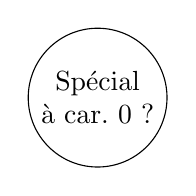
\begin{tikzpicture}\node[draw,circle,inner sep=2pt]{\shortstack{\unsure{Spécial}\\à car.\ 0 ?}};\end{tikzpicture}}
\deleted{définit un op. diff.}
\uline{se factorise de façon canonique en}
\diagram{\begin{tikzcd}[column sep=large]
\underline g \arrow[r,"{c=d^0}"] \arrow[rr,bend right=30,"D"'] & Z^1C_{S/R}(\underline g) \arrow[r,no head,"{\widetilde D}"] & M
\end{tikzcd}}

($\widetilde D$ est loc. induit par un op. diff. sur $\underline g\otimes\Omega^1_{S/R}$ ; \deleted{\unsure{donc les}} \inserted{\unsure{tous les}} $\Delta$, \deleted{\unsure{\Delta\text{ comme}}} \inserted{avec} $\Delta\circ d^0=D$, ont \unsure{$=$|même} restriction à $Z^1C_{\unsure{S}/R}(\underline g)$..)

Donc on trouve un composé
\diagram{\begin{tikzcd}[column sep=large]
\underline{\Gamma}(G) \arrow[r,"{g^{-1}dg}"] \arrow[rr,bend right=30,"{\unsure{\overset{\sim\!\sim}{D}|\widetilde D}}"'{draw,circle,inner sep=3pt}] & Z^1C_{S/R}(\underline g) \arrow[r,"{\widetilde D}"] & M
\end{tikzcd}}
\margin{220}

\scanpage{222}
1) Soit $f:X\longrightarrow S$ morphisme lisse d'espaces analytiques (lisses)

$\omega$ une 1-forme fermée \inserted{(holomorphe)} relative sur $X/S$

$a$ et $b$ deux sections \inserted{holomorphes} de $X$ sur $S$, telles que $\forall s\in S$, $a(s)$ et $b(s)$ \inserted{sont dans la \unsure{$=$|même}. comp. connexe de $X_s$}.

Localement sur $S$, on peut trouver un arc \deleted{diff.} \inserted{différentiable par morceaux} $C_s:[0,1]=I\longrightarrow X_s$, joignant $a(s)$ et $b(s)$, et dépendant continûment de $s$.

Utilisant le fait que $\omega$ est fermée, donc localement de la forme $d_{X/S}\varphi$, on constate que la fonction sur $S$
\[
I(s)=\int_{C_s}^{\deleted{\unsure{b(s)}}}\omega_s=\int_{a(s)}^{b(s)}\omega_s
\]
est holomorphe en $s$. [On \inserted{\unsure{se place} au voisinage de $s_0\in S$ et \unsure{se}} ramène au cas où \deleted{\unsure{a(s_0)\text{ et}}} $a(s_0)$ et $b(s_0)$ sont assez voisins pour que dans un ouvert $U$ contenant $a(s_0),b(s_0)$, on ait $\omega|U=d\varphi$, donc pour $s$ voisin de $s_0$, $I(s)=\varphi b(s)-\varphi a(s)$].

Changeant le système des $C_s$ revient à le remplacer par $C'_s=C_s+Z_s$, $Z_s$ un 1-cycle, donc on trouve
\[
(1)\qquad I'(s)=I(s)+\underbrace{\int_{Z_s}\omega_s}_{\deleted{\unsure{\Pi}}}
\]

Considérons une expression formelle (avec des $\omega_i$ comme $\omega$, et des op. diff. \inserted{(hol.)} $D_i$ sur $S$]
\[
(2)\qquad \sum D_{is}\int_{a(s)}^{b(s)}\omega_{is}
\]
\margin{221}

\scanpage{223}
Cette fonction est déterminée, indépendamment du choix de $C_s$, modulo une expression de la forme
\[
(3)\qquad \sum D_{is}\int_{Z_s}\omega_{is}\quad
\deleted{\unsure{=\int_{Z_s}\sum D_{is}\omega_{is}}}
\]
\deleted{(\uline{NB} Le fait que $Z_s$ est un \uline{1-cycle} permet de}

Supposons que les $D_i,\omega_i$ soient tels que l'expression précédente soit nulle, quelle que soit \deleted{\unsure{et}} la famille continue $s\longrightarrow Z_s$ de 1-cycles \deleted{$\unsure{Z}$} sur un ouvert de $S$. \deleted{Alors l'expression} \inserted{On dira} que \deleted{\unsure{les}} $\mu\unsure{=|:}(D_i,\omega_i)_{i\in I}$ \uline{définit une équation de Picard-Fuchs sur} $X/S$. Alors pour deux sections hol. \unsure{quelc.} $a,b$ de $X/S$, l'expression
\[
(4)\qquad \mu(a,b)=\sum_i D_{is}\int_{a(s)}^{b(s)}\omega_{is}
\]
est bien déterminée, et est une fonction holomorphe sur $S$. Bien sûr on aura
\[
(5)\qquad \mu(a,b)+\mu(b,c)=\mu(a,c).
\]

Cherchons une condition suffisante maniable, \inserted{\unsure{d'une forme diff.|d'une forme différentielle}} \deleted{pour} \deleted{un \unsure{critère}\inserted{\unsure{d'allure|faible}} \uuline{infinitésimal} et en plus global,} pour que $\mu$ soit de Pic. Fuchs. Notons
\margin{222}

\scanpage{224}
que \deleted{\unsure{par}} sur
\[
\boxed{(6)\quad \underline\Phi=f_*(Z\underline\Omega^1_{X/S})/df_*(\underline{\mathcal O}_X)},
\]
il y a une connexion intégrable naturelle, grâce à la formule de Cartan \unsure{---|.} les $\omega_i$ définissent des sections $\omega'_i$ de $\underline\Phi$, et l'on peut former les $D_i\deleted{\unsure{\omega}}\omega'_i$. Je dis qu'il suffit qu'on ait
\margin{attention, \unsure{ne} marche tel quel que si $X\longrightarrow S$ est steinien}
\[
(7)\qquad \sum D_i\omega'_i=0.
\]

Lorsque $X/S$ est muni d'une connexion intégrable, alors le calcul des $\sum D_i\omega'_i$ se fait ainsi : \inserted{$f_*(\underline\Omega^*_{X/S})$ sera aussi stratifié; donc} chaque $D_i$ se remonte \deleted{par la stratification en} \inserted{en un opérateur} $\overline D_i$ sur $\underline\Omega^*_X$ \inserted{commutant à la diff. rel. $d_{X/S}$} et \deleted{\unsure{comme}} \deleted{$\omega_i$ est une forme fermée} \deleted{on peut former}

\deleted{\[
\boxed{\begin{gathered}
(8)\qquad \alpha_{\overline D_i}\omega_i=\alpha_{\overline D_i^0}\omega_i+c_i\omega_i\\
\left\{\begin{aligned}
\overline D_i&=\overline D_i^0+c_i\,\mathrm{id}\qquad
\left(\begin{array}{l}\overline D_i^0\text{ à coeff. cts}\\c_i\text{ section de }\mathcal O_X\end{array}\right)\\
(9)\qquad \alpha_{\overline D_i^0}d\varphi&=\unsure{d}\overline D_i^0\varphi
\end{aligned}\right.
\end{gathered}}
\]}

Considérons alors
\[
(\unsure{8})\qquad \sum\deleted{\unsure{\alpha}}(\overline D_i)\omega_i=\overline\omega
\]
qui est encore une forme fermée.
On vérifie alors \inserted{aussitôt} que l'on a
\margin{223}

\scanpage{225}
\[
(9)\qquad \sum D_i\omega'_i=\overline\omega'\qquad\text{dans }\underline\Phi
\]
et la condition (7) signifie que l'on a, localement au dessus de $S$, une relation
\[
(10)\qquad \overline\omega\left(=\sum\overline D_{\deleted{\unsure{s}}i}\omega_i\right)=d\varphi,\qquad \varphi\in\Gamma(X,\mathcal O_X).
\]
Pour voir que cette relation implique bien la nullité de (3), il suffit de prouver
\[
(11)\qquad \sum_i D_{is}\int_{Z_s}\omega_{is}=\int_{Z_s}\overline\omega
\]
qui implique, si $\overline\omega=d\varphi$, que le premier mb est égal à $\int_{\partial Z_s}\varphi=0$ car $\partial Z_s=0$.

En fait, (11) provient de la relation générale
\[
(12)\qquad D_s\int_{Z_s}\omega_s=\int_{Z_s}\overline D_s\omega_s
\]
valable pour tt op. diff. hol. $D$ sur $S$, et tte forme \inserted{holomorphe fermée} $\omega_{\deleted{\unsure{i}}}$ sur $X$ [le fait que $\omega$ est fermée implique que $\int_{Z_s}\omega$ est fonction holomorphe en $s$, et donne un sens au premier mb de (12)]. Pour prouver cette
\margin{224}

\scanpage{226}
dernière, on \deleted{[peut se ramener, en décomposant $Z_{s_0}$ en \deleted{\unsure{des}} \inserted{petits} chemins $a_i^0\longrightarrow a_{i+1}^0$, et transportant \deleted{\unsure{par}} horizontalement les $a_i^0$, \deleted{\unsure{et}}]} va prouver la relation plus générale
\[
(13)\qquad D_s\int_{a(s)}^{b(s)}\omega_s=\int_{a(s)}^{b(s)}(\overline D\omega)_s,
\]
valable pour des limites d'intégration $a(s),b(s)$ qui sont des \uline{sections horizontales} pour la connexion. [NB. Bien entendu, on suppose, pour donner un sens à cette formule, qu'on choisit les \unsure{$=$|mêmes} $C_s$ aux deux mb, donc (13) s'écrit en tte précision
\[
(13\ \mathrm{bis})\qquad D_s\int_{C_s}\omega_s=\int_{C_s}(\overline D\omega)_s\qquad].
\]

Pour prouver (13), on se ramène, en \inserted{se plaçant au voisinage de $s_0\in S$ et} décomposant le domaine $\int_{a(s)}^{b(s)}$, au cas où $a(s_0),b(s_0)$ sont assez voisins, de sorte qu'on peut se placer dans un ouvert $U$ où l'on a $\omega=d\varphi$. Mais alors le $1^{\mathrm{er}}$ mb est $D_s(\varphi(b(s))-\varphi(a(s)))$, le
\margin{225}

\scanpage{227}
deuxième est
\[
\int_{a(s)}^{b(s)}\overline D\,d\varphi=\int_{a(s)}^{b(s)}d\,\overline D\varphi=(\overline D\varphi)(b(s))-(\overline D\varphi)(a(s)),
\]
\deleted{et les} et les deux expressions sont égales, grâce au fait que $a,b$ sont des sections horizontales. Notons aussi que ceci montre, si $a,b$ sont des sections \uline{horizontales}, qu'on aura
\[
(14)\qquad \mu(a,b)=\int_{a(s)}^{b(s)}\left(\sum\overline D_i\omega_i\right)_s=\varphi(b(s))-\varphi(a(s)),
\]
où $\varphi$ est \unsure{défini|définie} par la relation (10).

Prouvons la suffisance de (7) pour la nullité de (3) en général. On va prouver ``plus \unsure{généralement|précisément}'' qu'on aura alors
\[
\sum D_{is}\int_{C_s}\omega_{is}=0
\]
lorsque $C_s$ est un 1-cycle dans $X_s$, variant différentiablement avec $s$, dont le bord est ``horizontal'' en $s$, ou ce qui revient au même
\[
\sum_i D_{is}\int_{a(s)}^{b(s)}\omega_{is}=0
\]
si $a,b$ sont des sections \uline{horizontales} de $X$ sur \deleted{\unsure{S}} \inserted{un ouvert de $S$.} \deleted{Pour} Se plaçant au voisinage d'un
\margin{226}

\scanpage{228}
point $s_0\in S$ on est ramené encore au cas où $a(s_0)$ est proche de $b(s_0)$, de sorte qu'on peut \deleted{\unsure{donc}} se placer dans un ouvert de $X$ assez petit pour qu'il y ait une connexion. Et on gagne.

On peut aussi noter, \deleted{que} pour prouver la \deleted{formule} nullité de (3) comme conséquence de (7), que l'on a
\[
\deleted{(\unsure{15})}\qquad \sum D_{is}\int_{Z_s}\omega_i=\int_{Z_s}\left(\sum\overline D_i\omega'_i\right)_s
\]
où le deuxième mb a un sens, car $\int_{Z_s}\overline\omega_s=0$ si $\overline\omega_s$ est un bord, et $\left(\sum\overline D_i\omega'_i\right)_s$ est une forme définie modulo un bord. \uline{La formule \unsure{envisagée}} \deleted{équivaut} \inserted{revient à}
\[
(15)\qquad\boxed{D_s\int_{Z_s}\omega'_s=\int_{Z_s}(\overset{\deleted{\unsure{-}}}{D}\omega')_s}
\]
qui donne la propriété transcendante essentielle de la connexion intégrable canonique sur $\underline\Phi$. Nous n'allons pas prouver (15) ici, et l'admettrons, mais notons que
\margin{227}

\scanpage{229}
(15) nous donne une \uline{réciproque} pour la condition envisagée pour que $(D_i,\omega_i)$ soit de Picard-Fuchs : il f. et s. que l'on ait (7). Cela résulte du th. de De Rham sur les fibres $X_s$ ....

\uline{Calcul de} $\mu(a,b)$ par voie ``algébrique'', sans calcul d'intégrales. \inserted{C'est local sur $S$.} La formule (5) nous ramène à calculer $\mu(a,b)$ \inserted{au voisinage de $s_0$,} pour \deleted{$a,b$} $a(s_0)$ et $b(s_0)$ assez voisins. Cela nous permet alors de supposer que sur $X/S$ il y a une connexion intégrable. On peut \unsure{$=$|même} supposer, par un choix convenable, que les sections $a,b$ sont horizontales. Alors on trouve (14)
\[
\mu(a,b)=\varphi(b(s))-\varphi(a(s))
\]
où $\varphi$ est défini par (10).

Il y aurait lieu \unsure{d'expliciter|d'expliquer} aussi une formule explicite, sans supposer que $a(s)$ et $b(s)$ soient horizontales. Faisons le calcul au voisinage de $s_0$, et soient $a_0,b_0$ les
\margin{228}

\scanpage{230}
sections horizontales au voisinage de $s_0$, telles que
\[
a_0(s_0)=a(s_0),\quad b_0(s_0)=b(s_0).
\]
On a
\[
\mu(a,b)=\underbrace{\mu(a_0,b_0)}_{\deleted{\int_{a_0}^{b_0}\unsure{\varphi}}\;\varphi(b_0)-\varphi(a_0)}
+\mu(b_0,b)-\mu(a_0,a)
\]
donc
\[
\mu(a,b)(s_0)=\bigl[\varphi(b(s_0))-\varphi(a(s_0))\unsure{]|)}
+\left(\sum_i D_{is}\int_{b_0(s)}^{b(s)}\omega_{is}
-\sum_i D_{is}\int_{a_0(s)}^{a(s)}\omega_{is}\right)_{s=s_0}.
\]
Il faut calculer les deux termes de droite, c'est une histoire purement locale.

\deleted{Notons qu'on a, grâce à la connexion de $X/S$
\[
da\in\Gamma(S,a^*(\unsure{\mathcal T}_{X/S})\otimes\Omega^1_S)
\]
d'où en contractant avec
\[
a^{\unsure{*|\vee}}(\omega)\in\Gamma(S,\underbrace{a^*(\Omega^1_{X/S})}_{\text{dual de }a^{\unsure{*|\vee}}(\unsure{\mathcal T}_{X/S})})
\]
une section, que nous noterons $a^*(\omega)$
\[
a^*(\omega)\in\Gamma(S,\Omega^1_S)
\]
Cette \deleted{section} \inserted{forme} est encore \uline{fermée}, \inserted{$\omega$ l'étant} [N.B. pour le voir définir $a^{\unsure{*|\vee}}(\omega)$ pour tte forme (degré quelconque, fermée ou non) sur $X$, et noter que $a^*$ commute à la différentielle ext.)}
\margin{\unsure{donc une} \unsure{formule|forme} ....!}
\margin{229}

\scanpage{231}
\margin{\diagram{\begin{tikzcd}S\arrow[d]\\T\end{tikzcd}}}
\unsure{version relatif}
\margin{\figure{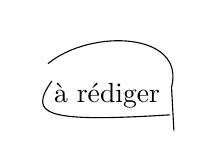
\begin{tikzpicture}[baseline=(n.base)]\node(n) at (0,0){\unsure{à rédiger}};\draw (0.85,-0.45)--(0.82,0.1) .. controls (1,0.8) and (-0.2,0.85) .. (-0.75,0.4);\draw (-0.7,0.18) .. controls (-1,-0.25) and (-0.8,-0.35) .. (0.8,-0.25);\end{tikzpicture}}}

1) Soit
\diagram{\begin{tikzcd}F\arrow[r,"D"]&G\arrow[r,"D'",no head]&H\end{tikzcd}}
une suite d'op. différentiels, qui est ``formellement exacte''. Alors pour tt $P$, la suite
\diagram{\begin{tikzcd}
\operatorname{Diff}^i(P,F)\arrow[r,"u\mapsto D\circ u"]&
\operatorname{Diff}^{i+1}(P,G)\arrow[r,"v\mapsto D'\circ v",no head]&
\operatorname{Diff}^{i+2}(P,H)
\end{tikzcd}}
est exacte, et la suite
\diagram{\begin{tikzcd}
\operatorname{Diff}^i(H,P)\arrow[r,"u\mapsto u\circ D'"]&
\operatorname{Diff}^{i+1}(G,P)\arrow[r,"u\mapsto u\circ D"]&
\operatorname{Diff}^{i+2}(F,P)
\end{tikzcd}}
est exacte.

2) Supposons que $E$ sur $S$ soit loc. libre \uline{stratifié}, et que le lemme de Poincaré formel soit vrai pour le complexe
\[
E\otimes\Omega^*_{S/T}=\Omega^*_{S/T}(E)
\]
[p.ex. $S$ lisse sur $T$, et caractéristiques de $T$ nulles].
Alors \inserted{$\forall\ P$ quelc. et $i\geq0$} la suite
\diagram{\begin{tikzcd}[column sep=large]
0 & \operatorname{Hom}(E,P)\arrow[l] &
\operatorname{Diff}^i(E,P)\arrow[l,"\deleted{\unsure{u\mapsto u(h)}}"']\arrow[d,"\sim"'] &
\operatorname{Diff}^{i-1}(\unsure{E}\otimes\Omega^1_{S/T},P)\arrow[l,"u\mapsto u\circ d_E^0"'] &
\cdots\arrow[l,"u\mapsto u\circ d_E^1"']\\
&\bigl[&\operatorname{Hom}(P^i(E),P)\arrow[ul,"u\mapsto u\circ\unsure{\delta_i^E}"']&\bigr]
\end{tikzcd}}
\inserted{où $\unsure{\delta_i^E}:E\to P^i(E)$ défini par la stratification}
est exacte.

\uline{NB} $\operatorname{Ker}(\operatorname{Diff}^i(E,P)\to\operatorname{Hom}(E,P))$ est désigné par
$\operatorname{Diff}^i_+(E,P)$, op. diff. ``à coeff. cts'' rel. à la stratification.
\margin{230}

\scanpage{232}
Donc on trouve

\uline{Corollaire}
\[
\operatorname{Diff}^{(i)}_+(E,P)\simeq
\operatorname{Diff}^{i-1}(E\otimes\Omega^1_{S/T},P)/\operatorname{Im}\operatorname{Diff}^{i-2}(E\otimes\unsure{\Omega_{S/T}|\Omega^2_{S/T}},\unsure{P})
\]
Par suite, on a un hom naturel \figure{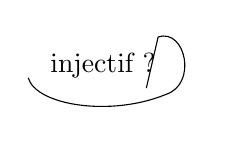
\begin{tikzpicture}[baseline=(n.base)]\node(n) at (0,0){injectif ?};\draw (0.7,0.37) .. controls (1.05,0.48) and (1.2,-0.23) .. (0.8,-0.36) .. controls (0.1,-0.65) and (-0.85,-0.5) .. (-0.95,-0.15);\draw (0.7,0.37)--(0.55,-0.28);\end{tikzpicture}}
\diagram{\begin{tikzcd}
\operatorname{Diff}^{(i)}_+(E,P)\arrow[r]&\operatorname{Hom}\mathrm{add}(\operatorname{Ker}d_E^1,P)
\end{tikzcd}}
\margin{l'image est \unsure{appelé|appelée}: faisceau des op. diff. de $\operatorname{Ker}d_E^1$ dans $P$}

Pour $i$ fixé, le $P$ ``universel'' pour les op. diff à coeff constants (d'ordre $\leq i$) sur $E$ est
\[
P^{(i)}(E)/\underline{O}_S.\delta_i^{\unsure{E}}(E),
\]
où
\[
\delta_i:E\longrightarrow P^i(E)
\]
est défini par la stratification.

3) Supposons maintenant donné un sous-Module $N$ de $E$, on s'intéresse aux hom ``différentiels'' $\operatorname{Ker}d_E^1\to P$ qui s'annulent sur $d_E^0N$, qui correspondent donc aux op. diff. $E\unsure{\mathbin{-}|\to}P$, à coeff. cts, et qui s'annulent sur $N$, donc aux op. diff. $M=E/N\unsure{\mathbin{-}|\to}P$ qui \deleted{sont ``\unsure{formels}''} deviennent à coeff. cts sur $E$. Ils correspondent \inserted{(pour l'ordre $\leq i$),} aux hom linéaires
\[
P^i(M)\longrightarrow P
\]
qui s'annulent sur $\rho_iE$; où
\[
\rho_i:E\unsure{\mathbin{-}|\to}P^i(M)
\]
\margin{231}

\scanpage{233}
est l'hom. composé [linéaire pour la structure \uline{gauche} sur $P^i(M)$]
\diagram{\begin{tikzcd}
E\arrow[r,"\delta_i"]&P^i(E)\arrow[r,no head]&P^i(M).
\end{tikzcd}}
Donc, pour $P$ variable, c'est représenté par
\[
\Phi_i=P^i(M)/\underline{O}_S.\rho_i(E),
\]
les $\Phi$ forment un syst. projectif strict, déterminé par la connaissance de $M$ et de
\[
\rho_\infty:E\longrightarrow P^\infty(M)
\]
(linéaire pour la structure \uline{gauche} de $P^\infty(M)$), défini par les $\rho_i$.
Attention, ici $\rho_\infty$ satisfait à des \deleted{\unsure{le}} conditions spéciales: \unsure{son} composé $E\to M$ avec l'augmentation $P^\infty(M)\to M$ est un épimorphisme, $+$ conditions d'intégrabilité ---
\margin{232}

\scanpage{234}
\uline{\mspage{1}}
\figure{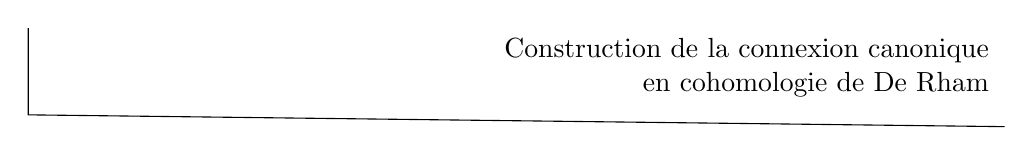
\begin{tikzpicture}[baseline=(n.base)]\node(n)[align=right,text width=12cm] at (0,0){Construction de la connexion canonique\\en cohomologie de De Rham};\draw (-6.2,0.5)--(-6.2,-0.6)--(6.2,-0.75);\end{tikzpicture}}

\diagram{\begin{tikzcd}[column sep=large]
X_0\arrow[d,"f_0"]&X'\arrow[d,"f'"]&X''\arrow[dl,"f''"]\\
T_0\arrow[r,hook,no head,"\substack{\text{immersion}\\1\text{-nilpotente}}"']&T
\end{tikzcd}}
\margin{schéma relatif \unsure{formellt.} lisse}
\margin{\figure{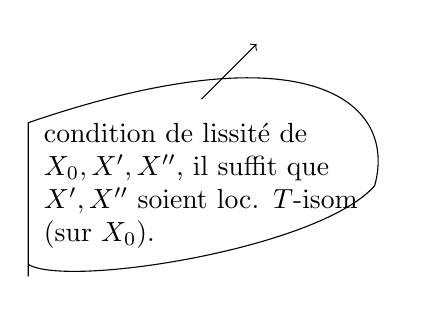
\begin{tikzpicture}[baseline=(n.base)]\node(n)[text width=4cm,align=left] at (0,0){\unsure{condition} de lissité \inserted{de $X_0,X',X''$}, \unsure{il} suffit que $X',X''$ soient loc. $T$-isom (sur $X_0$).};\draw (-2.2,-1.15)--(-2.2,0.8) .. controls (1.3,2) and (2.5,1.1) .. (2.2,0) .. controls (1.5,-0.8) and (-1.7,-1.3) .. (-2.2,-1);\draw[->] (0,1.1)--(0.7,1.8);\end{tikzpicture}}}
\[
T_0=V(\underline{I})
\]
\[
X'\mathbin{\times}_T T_0\xrightarrow{\sim}X_0\qquad
X''\mathbin{\times}_T T_0\simeq X_0
\]
$X',X''$ deux prolongements lisses de $X_0/T_0$ sur $T$.

\diagram{\begin{array}{lll}
\mathcal P&\text{faisceau sur esp }X_0\text{ des germes des}&T\text{-isom }X'\to X''\\
\mathcal G&\rule{8cm}{0.4pt}&T\text{-autom }X''\to X''
\end{array}}
alors
\[
\mathcal G\simeq\operatorname{Hom}(\Omega^1_{X_0/T_0},f_0^{\unsure{*}}(I))
=\unsure{\mathcal T}_{X_0/T_0}\otimes f_0^{\unsure{*}}(\underline I)
\]
$\mathcal P$ un \inserted{$\mathcal G$-torseur à droite} [faisceau principal homogène \inserted{à droite} sur $\mathcal G$.]

\diagram{\begin{tikzcd}
\mathcal P\mathbin{\times}\Omega^\bullet_{X'/T}\arrow[r]&\Omega^\bullet_{X''/T}
\end{tikzcd}}
i.e.
\diagram{\begin{tikzcd}
\mathcal P\arrow[r,"u"]&\underline{\operatorname{Isom}\text{ de complexes}}(\Omega^\bullet_{X'/T},\Omega^\bullet_{X''/T})
\end{tikzcd}}
\[
\subset Z^0\underline{\operatorname{Hom}}^\bullet(\Omega^\bullet_{X'/T},\Omega^\bullet_{X''/T})
\]
\diagram{\begin{tikzcd}
\mathcal G\arrow[r,"v"]&\underline{\unsure{\operatorname{Aut}}\text{ de complexes}}(\Omega^\bullet_{X''/T})
\end{tikzcd}}
\[
\subset Z^0\underline{\operatorname{Hom}}^\bullet(\Omega^\bullet_{X''/T},\Omega^\bullet_{X''/T})
\]
\diagram{\begin{tikzcd}
\mathcal G\arrow[r,"k"]&\underline{\operatorname{Hom}}^{(-1)}(\underline{\Omega}^\bullet_{X''/T},\Omega^\bullet_{X''/T})
\end{tikzcd}}
par procédés antérieurs

On a
\[
\left\{\begin{aligned}
u(pg)&=u(p)v(g)\qquad&\text{si }p&\in\Gamma(U,\mathcal P)\\
&&g&\in\Gamma(U,\mathcal G)\\
v(g)-\mathrm{id}&=dk(g)+k(g)d
\end{aligned}\right.
\]
\margin{233}

\scanpage{235}
\uline{\mspage{2}.}
Plus généralement, sur un espace \unsure{top} \inserted{annelé} $X$, soient $K',K''$ deux complexes de Modules, et
$\mathcal G$ un faisceau abélien

$\mathcal P$ un $\mathcal G$-torseur à droite
\diagram{\begin{tikzcd}
\mathcal P\arrow[r,"u",no head]&\unsure{Z^0}\underline{\operatorname{Hom}}^\bullet(K',K'')\\
\mathcal G\arrow[r,"v"]&\underline{\operatorname{Hom}}^\bullet(K'',K'')\\
\mathcal G\arrow[r,"\unsure{h|k}"]&\underline{\operatorname{Hom}}^{-1}(K^{\unsure{\prime|\prime\prime}},K'')
\end{tikzcd}}
\[
\begin{aligned}
u(pg)&=u(p)v(g)\\
v(g+g')&=v(g)+v(g')\\
u(g)&=d\unsure{h|k}(g)+\unsure{h|k}(g)d
\end{aligned}
\]
On veut en conclure un hom dans la cat. dérivée \inserted{$K'\to K''$} d'où
\[
R\Gamma_X(K')\longrightarrow R\Gamma_X(K'')
\]
(compatible avec la structure sur $\deleted{\unsure{R\Gamma_X}}\Gamma_X(\underline O_X)$ ....)
[et plus gén. en relativisant par rapport à un morphisme d'espaces annelés $X\unsure{\mathbin{-}|\to}T$ ...]

On introduit l'extension $\overline{\mathcal G}$ de $\mathbf Z$ par $\mathcal G$
\diagram{\begin{tikzcd}
0\arrow[r,no head]&\mathcal G\arrow[r,no head]&\overline{\mathcal G}\arrow[r,"j",no head]&\mathbf Z\arrow[r,no head]&0
\end{tikzcd}}
définie au moyen de $\mathcal P$ par la relation
\[
j^{-1}(1)\simeq\mathcal P\qquad(\text{isom de }\uline{$\mathcal G$-torseurs}\text{ ...})
\]
Soit
\[
\mathcal H=\underline{\operatorname{Hom}}^\bullet(K',K'')
\]
et soit $L$ le complexe
\diagram{\begin{tikzcd}
0\arrow[r]&0\arrow[r]&\overset{\text{``}L^0}{\mathcal G}\arrow[r,no head]&\overset{\text{``}L^1}{\overline{\mathcal G}}\arrow[r]&0\arrow[r]&0
\end{tikzcd}}
\margin{234}

\scanpage{236}
On trouve donc un homomorphisme
\[
\varphi:L^\bullet\longrightarrow\mathcal H^\bullet
\]
par
\diagram{\begin{tikzcd}[column sep=large]
\cdots\arrow[r,no head]&0\arrow[r,no head]&\mathcal G\arrow[r,"i"]\arrow[d,"\unsure{\varphi^{-1}}"']&\overline{\mathcal G}\arrow[r,no head]\arrow[d,"\varphi^0"]&0\arrow[r,no head]&\cdots\\
&\mathcal H^{-2}\arrow[r]&\mathcal H^{-1}\arrow[r,"\delta^{-1}",no head]&\mathcal H^0\arrow[r]&\mathcal H^1\arrow[r,no head]&\cdots
\end{tikzcd}}
défini par les conditions
\[
\varphi^{-1}=\unsure{h|k}\qquad\varphi^0\vert\mathcal P=\unsure{u|v}
\]
et la commutativité du carré

[\deleted{\unsure{On voit que}} Un hom de $\overline{\mathcal G}$ dans un un faisceau $F$ $=\{$Hom $v$ de $\mathcal G$ dans $F$, et hom $u$ de $\mathcal P$ dans $F$, avec condition $u(pg)=u(p)v(g)\}$.
Donc prenant $\deleted{\unsure{\delta\varphi^{-1}}}F=\mathcal H^0$, et $u,v$ comme dessus, on trouve $\varphi^0$, avec $\varphi^0i=u$. Mais
\[
u=\delta\deleted{\unsure{\varphi^{-1}}}\unsure{h|k}=\delta\varphi^{-1}\ \ldots
\]
]
Tensorisant avec $\underline O_X$, on trouve
\diagram{\begin{tikzcd}
\underline O_X\arrow[r,"\sim","\substack{\text{dans cat}\\\text{dérivée}}"']&\deleted{\unsure{L^\bullet}}\arrow[r]&\mathcal H\arrow[r]&R\underline{\operatorname{Hom}}(K',K'')
\end{tikzcd}}
dans
\deleted{On a donc}
\[
\boxed{\underline O_X\xrightarrow{\sim}R\underline{\operatorname{Hom}}(K',K'')\quad\text{ds cat. dérivée}}
\]
Donc
\diagram{\begin{tikzcd}
\deleted{\unsure{R\Gamma_X(L^\bullet)}}\arrow[r,"\sim",no head]&R\Gamma_X(\unsure{\underline O_X|\mathbf Z_X})\arrow[r]&\deleted{\unsure{R\Gamma_X\mathcal H}}\arrow[r]&R\operatorname{Hom}(K',K'')
\end{tikzcd}}
d'où
\[
\boxed{R\Gamma_X(\unsure{\underline O_X|\mathbf Z_X})\longrightarrow R\operatorname{Hom}(K',K'')}
\]
Par suite, \deleted{faisant} passant au $R\Gamma_X^0$, on trouve un élément de $R^0\operatorname{Hom}(K',K'')$, i.e. un hom de la cat. dérivée
\margin{235}

\cotefile{161-5}
\scanpage{3}
\begin{center}
Reprint of

\textit{Proceedings of a Conference on Local Fields}

\textit{NUFFIC Summer School held at Driebergen (The Netherlands) in 1966}

\rule{0.85\linewidth}{0.4pt}

\textbf{Springer-Verlag Berlin Heidelberg New York 1967}

\textbf{(Printed in The Netherlands). Not for Sale}

\textbf{Sur les groupes de Galois attachés aux groupes}

\textbf{$p$-divisibles}$^{1}$

J.-P. \textsc{Serre}
\end{center}
\margin{2}

\scanpage{4}
\begin{center}\textbf{Introduction}\end{center}

Soit $K$ un corps local de caractéristique 0 et de caractéristique résiduelle $p$, et soit $C$ la complétion d'une clôture algébrique de $K$. Soit $T$ le module de Tate ([9], n\textsuperscript{o} 2.4) associé à un groupe $p$-divisible $F$, défini sur l'anneau des entiers de $K$. \textsc{Tate} a montré ([9], \S\ 4, cor. 2 au th. 3) que $T\otimes C$ possède une décomposition analogue à celle de Hodge pour la cohomologie complexe. De nombreuses propriétés du module galoisien $T$ sont implicitement contenues dans cette décomposition. Dans son séminaire au Collège de France, résumé dans [8], \textsc{Tate} en a indiqué un certain nombre (notamment lorsque l'action du groupe de Galois est abélienne). Dans ce qui suit, j'explicite une autre conséquence de cette décomposition de $T\otimes C$: si $G$ est le groupe de Galois qui opère sur $T$, l'enveloppe algébrique de $G$ contient (sous une hypothèse de semi-simplicité convenable) un groupe «de Mumford-Tate» $p$-adique (\S\ 3, ths. 1 et 2). Lorsqu'on fait certaines hypothèses supplémentaires sur $F$, on en déduit que $G$ est \textit{ouvert} dans $\operatorname{Aut}(T)$ (cf. \S\ 5, th. 4). Ces hypothèses sont notamment vérifiées lorsque $F$ est un groupe formel à 1 paramètre, n'admettant pas de multiplication complexe formelle (\S\ 5, th. 5).

\begin{center}\textbf{\S\ 1. Enveloppes algébriques des groupes\par linéaires $p$-adiques}\end{center}

Soit $V$ un espace vectoriel de dimension finie sur le corps $p$-adique $\mathbf Q_p$, et soit $\operatorname{Aut}(V)$ le groupe de ses automorphismes, muni de sa structure

\footnotetext[1]{Le texte ci-dessous a été rédigé en décembre 1966. Il diffère de l'exposé oral par un plus grand usage de la théorie des groupes algébriques.

L'idée de remplacer les algèbres de Lie $p$-adiques par les groupes algébriques correspondants m'avait d'ailleurs été suggérée par Grothendieck il y a plusieurs années, en liaison avec sa théorie des «motifs».}
\margin{3}

\scanpage{5}
\begin{center}Sur les groupes de Galois attachés aux groupes $p$-divisibles\hfill119\end{center}

naturelle de groupe de Lie $p$-adique. Soit $G$ un sous-groupe compact de $\operatorname{Aut}(V)$. On sait (voir par exemple [7], p. 5.42) que $G$ est un \textit{sous-groupe de Lie} de $\operatorname{Aut}(V)$. Soit $\mathfrak g$ son algèbre de Lie; l'exponentielle définit un isomorphisme d'un voisinage ouvert de 0 dans $\mathfrak g$ (muni de la loi de groupe fournie par la formule de Hausdorff) sur un sous-groupe ouvert de $G$.

\textbf{Proposition 1.} -- \textit{Les conditions suivantes sont équivalentes:}

(a) \textit{$V$ est un $G$-module semi-simple.}

(b) \textit{$V$ est un $\mathfrak g$-module semi-simple.}

(c) \textit{$\mathfrak g$ est une algèbre de Lie réductive} (i.e. produit d'une algèbre abélienne $\mathfrak c$ par une algèbre semi-simple $\mathfrak s$) \textit{et $V$ est un $\mathfrak c$-module semi-simple.}

Soit $G_1$ un sous-groupe ouvert distingué de $G$ assez petit pour être contenu dans l'image de l'exponentielle. Tout sous-espace de $V$ stable par $\mathfrak g$ l'est aussi par $G_1$, et inversement. Cela montre l'équivalence de (b) et de la condition suivante:

(a$_1$) $V$ est un $G_1$-module semi-simple.

Mais $G/G_1$ est fini. On en déduit facilement (cf. \textsc{Chevalley} [1], tome III, p. 82, prop. 1) l'équivalence de (a) et (a$_1$). D'où $(\mathrm a)\Leftrightarrow(\mathrm b)$. L'équivalence $(\mathrm b)\Leftrightarrow(\mathrm c)$ est bien connue (\textsc{Bourbaki}, \textit{Gr. et Alg. de Lie}, chap. I, \S\ 6, n\textsuperscript{o} 5, th. 4).

Nous supposerons à partir de maintenant que les conditions de la prop. 1 sont vérifiées. Nous allons associer à $G$ un certain groupe algébrique réductif $G_{\mathrm{alg}}$, de la manière suivante:

Soit d'abord $\mathbf{GL}_V$ le $\mathbf Q_p$-groupe algébrique des automorphismes de $V$. Cela signifie, par définition, que, si $k$ est une $\mathbf Q_p$-algèbre commutative, le groupe $\mathbf{GL}_V(k)$ des points de $\mathbf{GL}_V$ à valeurs dans $k$ est égal à $\operatorname{Aut}(V\otimes k)$. En particulier, le groupe $\mathbf{GL}_V(\mathbf Q_p)$ s'identifie au groupe $\operatorname{Aut}(V)$ considéré plus haut.

\textbf{Définition.} -- \textit{On appelle enveloppe algébrique de $G$, et on note $G_{\mathrm{alg}}$, le plus petit sous-groupe algébrique de $\mathbf{GL}_V$ dont le groupe des points contienne $G$.}

L'existence et l'unicité de $G_{\mathrm{alg}}$ sont immédiates (et ne nécessitent aucune hypothèse sur $G$). Si $A$ est l'algèbre affine de $\mathbf{GL}_V$, l'idéal définissant $G_{\mathrm{alg}}$ est l'ensemble des $f\in A$ tels que $f(g)=0$ pour tout $g\in G$.

Utilisons maintenant l'hypothèse faite sur $G$. Décomposons l'algèbre de Lie $\mathfrak g$ en
\[
\mathfrak g=\mathfrak c\times\mathfrak s,
\]
où $\mathfrak c$ est le centre de $\mathfrak g$, et $\mathfrak s=[\mathfrak g,\mathfrak g]$ est semi-simple. On sait (\textsc{Chevalley}
\margin{4}

\scanpage{6}
120\hfill J.-P. \textsc{Serre}

[1], tome II, p. 177, th. 15) que $\mathfrak s$ est \textit{algébrique} (i.e. correspond à un groupe algébrique); si $\mathfrak c_{\mathrm{alg}}$ (resp. $\mathfrak g_{\mathrm{alg}}$) désigne la plus petite sous-algèbre de Lie algébrique de $\operatorname{End}(V)$ contenant $\mathfrak c$ (resp. contenant $\mathfrak g$), on a évidemment
\[
\mathfrak g_{\mathrm{alg}}=\mathfrak c_{\mathrm{alg}}\times\mathfrak s.
\]
L'algèbre $\mathfrak c_{\mathrm{alg}}$ est abélienne, et opère de façon semi-simple sur $V$. Il s'ensuit que $\mathfrak g_{\mathrm{alg}}$ est réductive. Le lien entre $\mathfrak g_{\mathrm{alg}}$ et $G_{\mathrm{alg}}$ est fourni par la proposition suivante:

\textbf{Proposition 2.} -- (i) \textit{L'algèbre de Lie de $G_{\mathrm{alg}}$ est $\mathfrak g_{\mathrm{alg}}$.}

(ii) \textit{$G_{\mathrm{alg}}$ est réductif} (\textsc{Mumford} [4], p. 26, déf. 1.4).

(iii) \textit{Toute composante connexe de $G_{\mathrm{alg}}$ rencontre $G$.}

Puisque $\mathfrak g_{\mathrm{alg}}$ est algébrique, il existe un sous-groupe algébrique connexe $H^0$ de $\mathbf{GL}_V$ d'algèbre de Lie $\mathfrak g_{\mathrm{alg}}$. Comme $\mathfrak g_{\mathrm{alg}}$ contient $\mathfrak g$, le groupe $H^0(\mathbf Q_p)$ contient un sous-groupe ouvert $G_1$ de $G$; on peut supposer $G_1$ distingué dans $G$. Soit $(g_i)$ un ensemble fini de représentants des classes de $G$ mod. $G_1$; la réunion $H$ des $H^0g_i$ est un sous-groupe algébrique de $\mathbf{GL}_V$ contenant $G$, et il est clair que c'est le plus petit possible. On a donc $H=G_{\mathrm{alg}}$, ce qui démontre (i) et (iii). L'assertion (ii) résulte de (i) (ou bien, si l'on préfère, du fait que $V$ est un $G_{\mathrm{alg}}$-module semi-simple et fidèle).

\textbf{Corollaire.} -- \textit{Si $\mathfrak c$ est algébrique, l'algèbre de Lie de $G_{\mathrm{alg}}$ est égale à $\mathfrak g$, et $G$ est un sous-groupe ouvert de $G_{\mathrm{alg}}(\mathbf Q_p)$.}

La première assertion est évidente; la seconde en résulte puisque $G$ et $G_{\mathrm{alg}}(\mathbf Q_p)$ sont des groupes de Lie $p$-adiques de même algèbre de Lie.

On peut donner une caractérisation des points de $G_{\mathrm{alg}}$ au moyen des \textit{invariants} du groupe $G$. Plus précisément, soient $r,s$ deux entiers $\geq0$, et soit $T_{r,s}(V)$ le produit tensoriel de $r$ copies de $V$ et de $s$ copies du dual $V^*$ de $V$. Le groupe $G$ opère (par transport de structure) sur $T_{r,s}(V)$; soit $T^0_{r,s}(V)$ le sous-espace de $T_{r,s}(V)$ formé des éléments invariants par $G$. Il est clair que $G_{\mathrm{alg}}$ laisse invariants les éléments de $T^0_{r,s}(V)$. De plus, cette propriété \textit{caractérise} les points de $G_{\mathrm{alg}}$:

\textbf{Proposition 3.} -- \textit{Soit $k$ une $\mathbf Q_p$-algèbre commutative, et soit $g\in\mathbf{GL}_V(k)$. Pour que $g$ appartienne à $G_{\mathrm{alg}}(k)$, il faut et il suffit que, pour tout couple $(r,s)$, l'extension $T_{r,s}(g)$ de $g$ à $T_{r,s}(V\otimes k)=T_{r,s}(V)\otimes k$ laisse invariants les éléments de $T^0_{r,s}(V)$.}

Notons d'abord qu'un élément de $T_{r,s}(V)$ est invariant par $G_{\mathrm{alg}}$ si et seulement si il appartient à $T^0_{r,s}(V)$. La prop. 3 est donc conséquence du lemme suivant:

\textbf{Lemme 1.} -- \textit{Soit $E$ un corps de caractéristique 0, soit $V$ un $E$-espace}
\margin{5}

\scanpage{7}
\begin{center}Sur les groupes de Galois attachés aux groupes $p$-divisibles\hfill121\end{center}

\textit{vectoriel de dimension finie, et soit $H$ un sous-groupe algébrique réductif de $\mathbf{GL}_V$. Pour qu'un point de $\mathbf{GL}_V$, à valeurs dans une extension de $E$, soit un point de $H$, il faut et il suffit que, pour tout couple $(r,s)$, il laisse invariants les éléments de $T_{r,s}(V)$ invariants par $H$.}

(En d'autres termes, un groupe réductif est déterminé par ses invariants tensoriels.)

Comme c'est là un résultat bien connu, je me bornerai à en esquisser la démonstration. On se ramène tout de suite au cas où le corps de base est algébriquement clos, ce qui permet d'identifier le groupe à l'ensemble de ses points rationnels; on peut aussi supposer que $H$ est contenu dans le groupe unimodulaire $\mathbf{SL}_V$ (en effet, si $n=\dim.V$, on remplace $V$ par $V\oplus\bigwedge^n V^*$). Soit alors $g$ un élément de $\mathbf{GL}_V$, vérifiant la condition du lemme, et n'appartenant pas à $H$. Du fait que $H$ est contenu dans $\mathbf{SL}_V$, $H$ et $Hg$ sont fermés dans $\operatorname{End}(V)$; puisque $H$ est réductif, il existe donc une fonction polynôme $f$ sur $\operatorname{End}(V)$, invariante par multiplication à gauche par $H$, et prenant les valeurs 0 sur $H$ et 1 sur $Hg$ (cf. [4], p. 29, cor. 1.2). Mais la représentation de $H$ dans $\operatorname{End}(V)$ par multiplication à gauche est isomorphe à la somme directe de $n$ copies de $V$. Comme $f$ appartient à l'algèbre symétrique du dual de $\operatorname{End}(V)$, l'hypothèse faite sur $g$ montre que $f$ est invariante par $g$. Mais c'est absurde, puisque $f(1)=0$ et $f(g)=1$.

\begin{center}\textbf{\S\ 2. Modules galoisiens du type de Hodge-Tate}\end{center}

A partir de maintenant, $K$ désigne un corps muni d'une valuation discrète, et complet pour la topologie définie par cette valuation. On note $A$ l'anneau des entiers de $K$, et $k=A/\mathfrak m$ le corps résiduel correspondant. On suppose $K$ de caractéristique zéro, et $k$ parfait de caractéristique $p$. On note $\overline K$ une clôture algébrique de $K$, et $C$ sa complétion. Le groupe de Galois $\operatorname{Gal}_K$ de $\overline K/K$ opère sur $C$ (cf. [9], \S\ 3).

Soit $\mathbf U_p=\mathbf Z_p^*$ le groupe des unités de $\mathbf Q_p$, et soit
\[
\chi:\operatorname{Gal}_K\to\mathbf U_p
\]
le caractère de $\operatorname{Gal}_K$ donnant l'action de ce groupe sur les racines $p^n$-èmes de l'unité. Par définition, on a
\[
sz=z^{\chi(s)}
\]
pour tout $s\in\operatorname{Gal}_K$ et pour toute racine de l'unité $z$ d'ordre une puissance de $p$.

Soit maintenant $X$ un $C$-espace vectoriel de dimension finie muni d'une

9\qquad Local Fields
\margin{6}

\scanpage{8}
122\hfill J.-P. \textsc{Serre}

loi d'opération de $\operatorname{Gal}_K$ continue et semi-linéaire; on a
\[
s(cx)=s(c)s(x)\quad\text{si}\quad s\in\operatorname{Gal}_K,\ c\in C,\ x\in X.
\]
Si $i\in\mathbf Z$, notons $X^i$ le sous-ensemble de $X$ formé des éléments $x$ tels que
\[
sx=\chi(s)^i x\quad\text{pour tout}\quad s\in\operatorname{Gal}_K;
\]
c'est un $K$-espace vectoriel. Posons $X(i)=X^i\otimes_K C$. L'injection $X^i\to X$ se prolonge en une application $C$-linéaire
\[
\varepsilon_i:X(i)\to X.
\]
\textsc{Tate} (séminaire au Collège de France) a démontré le résultat suivant:

\textbf{Proposition 4.} -- \textit{Soit $\sum X(i)$ la somme directe des $X(i)$. L'homomorphisme}
\[
\varepsilon:\sum X(i)\to X,
\]
\textit{somme des $\varepsilon_i$, est injectif.}

Rappelons brièvement la démonstration. Soit $(x_{ij})$ une base de $X^i$ sur $K$. Si $\varepsilon$ n'était pas injectif, il existerait des $c_{ij}\in C$, non tous nuls, tels que
\[
\sum c_{ij}x_{ij}=0.
\]
Parmi toutes les relations de ce genre, choisissons-en une de longueur minimum, et telle que $c_{i_0j_0}=1$ pour un couple $(i_0,j_0)$ particulier. Si $s\in\operatorname{Gal}_K$, on a
\[
\sum s(c_{ij})s(x_{ij})=0,
\]
d'où
\[
\sum s(c_{ij})\chi(s)^i x_{ij}=0.
\]
Utilisant la minimalité de la relation $(c_{ij})$, on en déduit que:
\[
s(c_{ij})\chi(s)^i=\chi(s)^{i_0}c_{ij},\quad\text{pour tout}\quad s\in\operatorname{Gal}_K.
\]
Mais, d'après \textsc{Tate} [9], \S\ 3, cette dernière relation entraîne $c_{ij}=0$ pour $i\neq i_0$, et $c_{ij}\in K$ pour $i=i_0$, contrairement au fait que les $(x_{ij})$ sont linéairement indépendants sur $K$. D'où la proposition.

La proposition précédente permet \textit{d'identifier $\sum X(i)$ à un sous-espace vectoriel de $X$}. Si ce sous-espace est égal à $X$ tout entier, nous dirons que $X$ est \textit{du type Hodge-Tate}, ou admet une décomposition de type (HT).

\textbf{Remarque.} Si $X$ est de type (HT), il en est de même de son dual $X^*$, et l'on a:
\[
X^*(i)=X(-i)^*;
\]
la vérification est immédiate. De même, tout produit tensoriel de modules galoisiens de type (HT) est de type (HT).
\margin{7}

\scanpage{9}
\begin{center}Sur les groupes de Galois attachés aux groupes $p$-divisibles\hfill123\end{center}

\begin{center}\textbf{\S\ 3. Le groupe de Mumford-Tate $p$-adique}\end{center}

Les notations étant celles du \S\ 2, soit $V$ un $\mathbf Q_p$-espace vectoriel de dimension finie muni d'une loi d'opération de $\operatorname{Gal}_K$ continue et linéaire. Soit $G$ l'image de $\operatorname{Gal}_K$ dans $\operatorname{Aut}(V)$; c'est un sous-groupe compact de $\operatorname{Aut}(V)$.

Faisons les deux hypothèses suivantes:

(H.1) -- \textit{$V$ est un $G$-module semi-simple.}

(H.2) -- \textit{Le module galoisien $V_C=V\otimes_{\mathbf Q_p}C$ est du type Hodge-Tate.}

(Précisons que $\operatorname{Gal}_K$ opère sur $V_C$ par transport de structure, i.e. par la formule $s(v\otimes c)=s(v)\otimes s(c)$.)

L'hypothèse (H.1) permet d'appliquer à $G$ les définitions et résultats du \S\ 1; en particulier, le groupe $G_{\mathrm{alg}}$ est défini. On notera que $G_{\mathrm{alg}}(C)$ est un sous-groupe du groupe $\operatorname{Aut}(V_C)$ des automorphismes $C$-linéaires de $V_C$.

Soit d'autre part $\lambda\in C^*$; notons $\varphi(\lambda)$ l'automorphisme de $V_C$ qui est l'homothétie de rapport $\lambda^i$ sur la $i$-ème composante $V_C(i)$ de $V_C$ (au sens du \S\ 2). On définit ainsi un homomorphisme $\varphi:C^*\to\operatorname{Aut}(V_C)$. Soit $\Phi=\operatorname{Im}(\varphi)$; c'est un sous-groupe de $\operatorname{Aut}(V_C)$.

\textbf{Théorème 1.} -- \textit{Le groupe $\Phi$ est contenu dans $G_{\mathrm{alg}}(C)$.}

Soit $(r,s)$ un couple d'entiers $\geq0$, et soit $W=T_{r,s}(V)$. Vu la prop. 3, il suffit de prouver que tout élément de $W$ invariant par $\operatorname{Gal}_K$ est invariant par $\Phi$ (lorsqu'on l'identifie à un élément de $T_{r,s}(V_C)=W_C$). Or:

(a) \textit{$W_C$ est du type Hodge-Tate.}

(b) \textit{Si $\lambda\in C^*$, l'action de $\varphi(\lambda)$ sur $W_C$ est donnée par:}
\[
\varphi(\lambda)x=\lambda^i x\quad\textit{si}\quad x\in W_C(i).
\]
En effet, (a) et (b) sont vrais pour $W=V$ (i.e. $r=1,s=0$), et, si elles sont vraies pour $W_1$ et $W_2$, elles le sont aussi pour $W_1^*$ et $W_1\otimes W_2$, en vertu de la remarque de la fin du \S\ 2.

Ceci étant, si $w\in W$ est invariant par $\operatorname{Gal}_K$, $w$ appartient \textit{a fortiori} à $W_C^0$, donc aussi à $W_C(0)=W_C^0\otimes_K C$, et (b) montre que $\varphi(\lambda)w=w$ pour tout $\lambda\in C^*$. L'élément $w$ est donc bien invariant par $\Phi$, cqfd.

Soit $M$ le plus petit sous-groupe algébrique de $\mathbf{GL}_V$ (au sens strict du terme, i.e. «défini sur $\mathbf Q_p$») dont le groupe des points à valeurs dans $C$ contienne $\Phi$. Je dirai que $M$ est \textit{le groupe de Mumford-Tate} du module galoisien $V$ (c'est en effet l'analogue $p$-adique de celui défini dans [5]). Le théorème 1 est visiblement équivalent au suivant:

\textbf{Théorème 2.} -- \textit{Le groupe $G_{\mathrm{alg}}$ contient le groupe $M$.}
\margin{8}

\scanpage{10}
124\hfill J.-P. \textsc{Serre}

\textbf{Remarques.} 1) Le groupe $\Phi$ est un $C$-sous-groupe algébrique connexe de $\mathbf{GL}_V(C)$. Il en résulte que $M$ est connexe, donc \textit{contenu dans la composante neutre} de $G_{\mathrm{alg}}$.

2) Soit $d\varphi$ l'endomorphisme de $V_C$ qui est l'homothétie de rapport $i$ sur $V_C(i)$. Les théorèmes 1 et 2, traduits en termes d'algèbres de Lie, signifient que:
\[
d\varphi\in\mathfrak g_{\mathrm{alg}}\otimes C.
\]

3) Soit $K_{nr}$ l'extension non ramifiée maximale de $K$ contenue dans $\overline K$. L'image $I$ de $\operatorname{Gal}(\overline K/K_{nr})$ dans $G$ est le \textit{sous-groupe d'inertie} de $G$. Comme $I$ est distingué dans $G$, $V$ est un $I$-module semi-simple et le groupe $I_{\mathrm{alg}}$ est défini. \textit{On a $M\subset I_{\mathrm{alg}}$}; cela se voit en appliquant le th. 2 sur le corps de base $\widehat K_{nr}$ complété de $K_{nr}$. (On n'aurait donc rien perdu si l'on avait supposé le corps résiduel $k$ algébriquement clos.)
\margin{En fait, on a $M=I_{\mathrm{alg}}$ (Sen)}

\begin{center}\textbf{\S\ 4. Un cas particulier}\end{center}

Conservons les notations des \S\S\ 2, 3, et faisons sur $V$ les hypothèses suivantes:

(H*.1) \textit{$V$ est un $\mathfrak g$-module absolument simple.}

(H*.2) \textit{$V_C$ est somme directe de $V_C(0)$ et $V_C(1)$.}

(H*.3) \textit{Les dimensions $n_0$ et $n_1$ de $V_C(0)$ et $V_C(1)$ sont $\geq1$ et premières entre elles.}

\textbf{Remarques.} -- 1) Les hypothèses (H*.1) et (H*.2) entraînent évidemment les hypothèses (H.1) et (H.2) du \S\ 3.

2) (H*.1) équivaut à dire que le $\mathfrak g$-module $V$ est \textit{semi-simple} et que \textit{son commutant est réduit aux homothéties} (\textsc{Bourbaki}, \textit{Alg.} VIII, \S\ 13, n\textsuperscript{o} 4, cor. à la prop. 5). En particulier, si $\mathfrak c$ désigne le centre de $\mathfrak g$, on voit que $\mathfrak c$ est, ou bien réduit à 0, ou bien égal à l'ensemble des homothéties de $V$. Dans les deux cas, c'est une algèbre de Lie algébrique, et l'on a donc $\mathfrak g_{\mathrm{alg}}=\mathfrak g$.

\textbf{Théorème 3.} -- \textit{Sous les hypothèses ci-dessus, on a $G_{\mathrm{alg}}=\mathbf{GL}_V$.}

Vu la remarque 2) ci-dessus, cet énoncé équivaut à:

\textbf{Corollaire 1.} -- \textit{L'algèbre de Lie $\mathfrak g$ de $G$ est égale à $\operatorname{End}(V)$.}

Il équivaut aussi à:

\textbf{Corollaire 2.} -- \textit{Le groupe $G$ est un sous-groupe ouvert de $\operatorname{Aut}(V)$.}

(En d'autres termes, l'action de $\operatorname{Gal}_K$ sur $V$ est aussi peu triviale que possible.)

\textbf{Démonstration.} -- Posons, pour simplifier $E=V_C$, $E_0=V_C(0)$ et
\margin{9}

\scanpage{11}
Sur les groupes de Galois attachés aux groupes $p$-divisibles\hfill 125

$E_1=V_C(1)$. Soit $H$ la composante neutre du $C$-groupe algébrique $G_{\mathrm{alg}}(C)$ (du fait que $C$ est algébriquement clos, nous nous permettons d'identifier un $C$-groupe algébrique à l'ensemble de ses points rationnels). Tout revient à montrer que $H=\mathbf{GL}_E$. Or, $H$ jouit des trois propriétés suivantes:

(a) \textit{$H$ est un sous-groupe réductif connexe de $\mathbf{GL}_E$, de commutant réduit aux homothéties.}

(b) \textit{$H$ contient le groupe $\Phi$ formé des automorphismes de $E$ qui sont l'identité sur $E_0$ et une homothétie sur $E_1$.}

Cela résulte du théorème 1.

(c) \textit{Les dimensions $n_0$ et $n_1$ de $E_0$ et $E_1$ sont premières entre elles.}

Le théorème 3 est donc une conséquence du résultat suivant, qui est un pur énoncé de théorie des groupes algébriques:

\textbf{Proposition 5.} -- \textit{Tout sous-groupe algébrique $H$ de $\mathbf{GL}_E$ vérifiant les conditions (a), (b), (c) ci-dessus est égal à $\mathbf{GL}_E$.}

La démonstration comporte plusieurs étapes:

1) Soit $T$ (resp. $S$) la composante neutre du centre de $H$ (resp. son groupe des commutateurs). On a $H=T\cdot S$, $T\cap S$ est fini, et $S$ est semi-simple. Vu (a), $T$ est, soit réduit à $\{1\}$, soit égal au groupe $\mathbf G_m$ des homothéties. Dans le premier cas, $H=S$ serait contenu dans le groupe unimodulaire $\mathbf{SL}_E$, ce qui est absurde car les éléments de $\Phi$ ne sont pas tous de déterminant 1. On a donc $T=\mathbf G_m$ et il va nous suffire de prouver que $S=\mathbf{SL}_E$.

2) Soit $\Theta$ le tore de dimension 2 formé des automorphismes de $E$ qui sont égaux à une homothétie sur $E_0$ et à une autre homothétie sur $E_1$. On a $\Theta=\mathbf G_m\cdot\Phi$, d'où $\Theta\subset H$ d'après ce qui précède. Soit $\psi:C^*\to\Theta$ l'homomorphisme défini par:
\[
\begin{array}{lll}
\psi(\lambda)x=\lambda^{n_1}x&\text{si}&x\in E_0\\
\psi(\lambda)x=\lambda^{-n_0}x&\text{si}&x\in E_1.
\end{array}
\]

On a $\det\psi(\lambda)=\lambda^{n_0n_1-n_1n_0}=1$ pour tout $\lambda\in C^*$. L'image $\Psi$ de $\psi$ est donc un sous-groupe connexe de $H\cap\mathbf{SL}_E$, donc aussi un sous-groupe de $S$.

3) Montrons maintenant que $S$ est \textit{simple} (i.e. tout sous-groupe algébrique distingué de $S$ est, soit fini, soit égal à $S$). Sinon, en effet, on aurait $S=(S'\times S'')/N$, avec $S'$, $S''$ semi-simples non réduits à $\{1\}$, et $N$ sous-groupe fini du centre de $S'\times S''$. Le $(S'\times S'')$-module $E$ peut s'écrire comme produit tensoriel:
\[
E=E'\otimes E'',
\]
\margin{10}

\scanpage{12}
126\hfill J.-P. \textsc{Serre}

 où $E'$ (resp. $E''$) est un $S'$-module (resp. $S''$-module) absolument simple. Soit $\widetilde\Psi$ la composante neutre de l'image réciproque de $\Psi$ dans $S'\times S''$. C'est un tore de dimension 1, donc isomorphe au groupe $\mathbf G_m$. Choisissons un isomorphisme $\sigma:\widetilde\Psi\to\mathbf G_m$. Notons respectivement $f$, $f_0$, $f_1$, $f'$, $f''$ les caractères des représentations $E$, $E_0$, $E_1$, $E'$, $E''$ de $\widetilde\Psi$. Ce sont des polynômes à coefficients entiers positifs en $\sigma$ et $\sigma^{-1}$. On a
\[
f'\cdot f''=f=f_0+f_1
\]
et
\[
f_0=n_0\sigma^a,\quad f_1=n_1\sigma^b,\quad\text{avec}\quad a,b\in\mathbf Z.
\]

On a $a\ne b$; sinon, en effet, $\Psi$ opèrerait sur $E$ par homothéties. De plus:
\[
f=n_0\sigma^a+n_1\sigma^b.
\]

Mais on vérifie tout de suite qu'un tel binôme ne peut se décomposer en produit de deux polynômes à coefficients entiers $\geq0$ que de façon triviale, l'un des facteurs étant un monôme $c\sigma^d$. L'entier $c$ doit diviser $n_0$ et $n_1$, donc doit être égal à 1 vu l'hypothèse $\operatorname{pgcd}(n_0,n_1)=1$. On a donc, par exemple, $f'=\sigma^d$, d'où $\dim.E'=1$. Mais c'est absurde, car l'image de $S'$ dans $S$ opèrerait trivialement sur $E$, contrairement au fait que $E$ est un $S$-module fidèle. Le groupe $S$ est donc bien un groupe \textit{simple}.

4) Soit $h=n_0+n_1$ la dimension de $E$, et soit $\mu_h$ le groupe des racines $h$-èmes de l'unité. On a $\lambda^{n_1}=\lambda^{-n_0}$ si $\lambda\in\mu_h$. L'homomorphisme $\psi$ de 2) transforme donc $\lambda\in\mu_h$ en une \textit{homothétie}. Comme $n_0$ et $n_1$ sont premiers entre eux, $\psi$ est injectif. On en conclut finalement que $\Psi$, donc \textit{a fortiori} $S$, \textit{contient le groupe $\mu_h$}, identifié à un sous-groupe du groupe des homothéties. En particulier, \textit{$\mu_h$ est contenu dans le centre de $S$}.

5) Vu 3) et 4), il ne nous reste plus qu'à démontrer le lemme suivant:

\textbf{Lemme 2.} -- \textit{Soit $S$ un groupe algébrique simple, et soit $\varrho:S\to\mathbf{GL}_E$ une représentation linéaire non triviale de $S$, de dimension $h$. Si le centre de $S$ est d'ordre multiple de $h$, $\varrho$ est un isomorphisme de $S$ sur $\mathbf{SL}_E$.}

Distinguons deux cas:

 a) Le groupe $S$ est de type $\mathbf A_n$ (au sens de la classification des groupes algébriques simples), donc quotient de $\mathbf{SL}(n+1)$ par un sous-groupe de son centre. Par hypothèse, $h$ divise $n+1$. D'où $\dim.S\geq\dim.\mathbf{SL}_E$, et, comme le noyau de $\varrho$ est fini, on en conclut d'abord que $\varrho$ applique $S$ sur $\mathbf{SL}_E$, puis que c'est un isomorphisme ($\mathbf{SL}_E$ étant simplement connexe).

 b) Le groupe $S$ n'est pas de type $\mathbf A_n$. La classification des groupes simples montre alors que le centre de $S$ a au plus 4 éléments. D'où $h\leq4$. Le cas $h=1$ est impossible. Le cas $h=2$ donnerait $S=\mathbf{SL}(2)$, qui est exclu.
\margin{11}

\scanpage{13}
Sur les groupes de Galois attachés aux groupes $p$-divisibles\hfill 127

Le cas $h=3$ n'est possible que si $S$ est de type $\mathbf E_6$; mais la dimension de $\mathbf E_6$ est bien trop grande pour que ce groupe puisse être plongé dans $\mathbf{SL}(3)$. De même, le cas $h=4$ n'est possible que pour un groupe de type $\mathbf D_n$, avec $n\geq4$ (pour $n\leq3$, $\mathbf D_n$ est, soit isomorphe à $\mathbf A_n$, soit non simple); comme la dimension de $\mathbf D_4$ est strictement supérieure à celle de $\mathbf{SL}(4)$, on conclut comme précédemment.

Ceci achève la démonstration du lemme 2, et, avec elle, celles de la prop. 5 et du th. 3.

\textbf{Remarque.} Même lorsqu'on ne fait plus l'hypothèse (H*.3), l'existence dans $S$ d'un tore $\Psi$ de dimension 1, ayant pour caractère un binôme $n_0\sigma^a+n_1\sigma^b$, peut être utilisée pour déterminer (au moins en partie) la structure de $S$.

\begin{center}\textbf{\S\ 5. Application aux groupes $p$-divisibles}\end{center}

Conservons les notations des paragraphes précédents. Soit $F$ un \textit{groupe $p$-divisible de hauteur $h$} sur l'anneau $A$ des entiers de $K$ (pour tout ce qui concerne les groupes $p$-divisibles, voir [9]). Soit $T$ le module de Tate de $F$, et soit $V=T\otimes\mathbf Q_p$. On sait ([9], n\textsuperscript{o} 2.4) que $\dim.V=h$, et que $\operatorname{Gal}_K$ opère continûment sur $T$ et sur $V$.

Nous aurons besoin de deux des principaux résultats de la théorie de Tate. Tout d'abord la décomposition de $V_C$ ([9], \S\ 4, cor. 2 au th. 3):

\textbf{Proposition 6.} -- \textit{$V_C=V\otimes C$ possède une décomposition de Hodge-Tate de la forme:}
\[
V_C=V_C(0)\oplus V_C(1).
\]
\textit{De plus, la dimension $n_1$ (resp. $n_0$) de $V_C(1)$ (resp. de $V_C(0)$) est égale à la dimension de la composante neutre de $F$ (resp. de son dual $F'$).}

(Rappelons, cf. [9], n\textsuperscript{o} 2.2, que la composante neutre $F^0$ de $F$ peut être identifiée à un \textit{groupe formel} sur $A$, au sens de \textsc{Dieudonné}, \textsc{Lazard}, \textsc{Lubin}; par la «dimension» de $F^0$, on entend le «nombre de paramètres» du groupe formel en question.)

Si $K'$ est une extension finie de $K$, d'anneau de valuation $A'$, notons $\operatorname{End}_{A'}(F)$ l'anneau des endomorphismes du groupe $p$-divisible $F\times_A A'$ déduit de $F$ par extension des scalaires de $A$ à $A'$. Soit $\operatorname{End}(F)$ la limite inductive (qui est en fait une réunion) des $\operatorname{End}_{A'}(F)$ lorsque $K'$ parcourt toutes les sous-extensions finies de $\overline K$ (cf. \textsc{Lubin} [2] pour le cas de dimension 1).
\margin{12}

\scanpage{14}
128\hfill J.-P. \textsc{Serre}

\textbf{Proposition 7.} -- (a) \textit{Le commutant de $G$ dans $T$ est égal à $\operatorname{End}_A(F)$.}

(b) \textit{Le commutant de $G$ dans $V$ est égal à $\operatorname{End}_A(F)\otimes\mathbf Q_p$.}

(c) \textit{Le commutant de $\mathfrak g$ dans $V$ est égal à $\operatorname{End}(F)\otimes\mathbf Q_p$.}

L'assertion (a) est démontrée dans [9], \S\ 4, cor. 1 au th. 4; (b) résulte de (a) par produit tensoriel avec $\mathbf Q_p$. Enfin, (c) résulte de (b) et du fait que le commutant de $\mathfrak g$ dans $V$ est égal à la réunion des commutants des sous-groupes ouverts de $G$.

Nous pouvons maintenant appliquer le théorème 3. On en tire:

\textbf{Théorème 4.} -- \textit{Faisons sur $F$ les hypothèses suivantes:}

(a) \textit{$V$ est un $G$-module semi-simple.}

(b) $\operatorname{End}(F)=\mathbf Z_p$.

(c) \textit{Les dimensions $n_1$ et $n_0$ de $F$ et de son groupe dual $F'$ sont $\geq1$ et premières entre elles.}

\textit{On a alors $G_{\mathrm{alg}}=\mathbf{GL}_V$, $\mathfrak g=\operatorname{End}(V)$ et $G$ est un sous-groupe ouvert de $\operatorname{Aut}(V)$.}

En effet, (H*.1) résulte de (a) et (b), compte tenu de la prop. 7, et (H*.2) et (H*.3) résultent de la prop. 6 et de (c).

\textbf{Remarque.} Les hypothèses (a), (b), (c) entraînent que $F$ est connexe (c'est donc un \textit{groupe formel}). En effet, si $F^0$ désigne la composante neutre de $F$, $V(F^0)$ est un sous-espace de $V(F)=V$ stable par $G$. Vu (a) et (b), on a donc $V(F^0)=0$ ou $V(F^0)=V$. Le premier cas entraîne $F^0=0$, d'où $n_1=0$, ce qui est exclu d'après (c). Le second cas entraîne $F=F^0$. De même, le dual de $F$ est un groupe formel.

Nous allons maintenant appliquer le théorème 4 aux \textit{groupes formels de dimension 1} (au sens de \textsc{Lubin} [2], [3]), i.e. au cas $n_1=1$. On a tout d'abord:

\textbf{Proposition 8.} -- \textit{Supposons $F$ connexe et de dimension 1. Pour tout $z\in V$, $z\ne0$, on a $\mathfrak g\cdot z=V$. En particulier, $V$ est un $\mathfrak g$-module simple.}

Par hypothèse, l'algèbre affine de $F$ est isomorphe à l'algèbre des séries formelles $A[[X]]$. Choisissons un tel isomorphisme (ce qui revient à considérer $F$ comme un groupe formel). La multiplication par $p$ dans $F$ est donnée par une série formelle
\[
f(X)=\sum_{n=1}^{\infty}a_nX^n,\qquad a_n\in A,\quad a_1=p.
\]
Puisque $F$ est de hauteur $h$, on a
\[
a_n\in\mathfrak m\quad\text{pour }n<p^h,\quad\text{et}\quad a_n\notin\mathfrak m\quad\text{pour }n=p^h,
\]
cf. \textsc{Lubin} [2].
\margin{13}

\scanpage{15}
Sur les groupes de Galois attachés aux groupes $p$-divisibles\hfill 129

Soit $\overline A$ (resp. $\overline{\mathfrak m}$) l'anneau (resp. l'idéal) de valuation de $\overline K$. Pour tout entier $n\geq0$, notons $f^{(n)}$ le $n$-ème itéré de $f$ (i.e. \textit{la multiplication par $p^n$} dans $F$), et soit $T_n$ l'ensemble des $x\in\overline{\mathfrak m}$ tels que $f^{(n)}(x)=0$. On sait (cf. par exemple [3]) que $T_n$ est un groupe (pour la loi de groupe formel définissant $F$), et que ce groupe est isomorphe à $(\mathbf Z/p^n\mathbf Z)^h$; on a $T=\varprojlim T_n$. Notons $T'_n$ l'ensemble des éléments de $T_n$ d'ordre $p^n$; on a
\[
T'_n=T_n-T_{n-1}.
\]

\textbf{Lemme 3.} -- \textit{Il existe un nombre $c>0$ tel que, pour tout $n\geq1$, et tout $x\in T'_n$, l'indice de ramification de l'extension $K(x)/K$ soit $\geq c\cdot p^{nh}$.}

Admettons provisoirement ce lemme, et démontrons la prop. 8. Quitte à transformer $z$ par une homothétie, on peut supposer que $z\in T$ et $z\notin pT$. Pour tout $n\geq1$, l'image $z_n$ de $z$ dans $T/p^nT=T_n$ appartient à $T'_n$. Soit d'autre part $U=G\cdot z$ \textit{l'orbite} de $z$ par $G$. C'est une \textit{sous-variété analytique $p$-adique} de $T$ et son espace tangent au point $z$ est égal à $\mathfrak g\cdot z$ (cf. par exemple [7], LG, p. 4.12). D'autre part, l'image $U_n$ de $U$ dans $T/p^nT$ est égale à $G\cdot z_n$, ensemble des conjugués de $z_n$. Mais, d'après le lemme 3, on a $\operatorname{Card}(G\cdot z_n)=[K(z_n):K]\geq c\cdot p^{nh}$. D'où
\[
\operatorname{Card}(U_n)\geq c\cdot p^{nh}.
\]

Soit alors $\mu$ la mesure de Haar de $T$, normalisée de telle sorte que $\mu(T)=1$. La formule ci-dessus entraîne que $\mu(U)\geq c$. Mais il est immédiat qu'une sous-variété analytique $p$-adique de $T$ n'a une mesure $>0$ que si son intérieur est non vide. Comme $U$ est une orbite, on en conclut que $U$ est \textit{ouvert} dans $T$. Son espace tangent en $z$ est donc $V$ tout entier. D'où $\mathfrak g\cdot z=V$.

\textit{Reste à démontrer le lemme 3.} Soit $v$ la valuation de $\overline K$, normalisée de telle sorte que $v(p)=1$. Soit $c_1$ la borne inférieure des $v(a_n)$, pour $n<p^h$. D'après ce qui a été dit plus haut, on a $c_1>0$. Soit $\varphi:\mathbf R_+\to\mathbf R_+$ l'application donnée par la formule
\[
\varphi(\alpha)=\operatorname{Inf}(p^h\alpha,\alpha+c_1).
\]

C'est une bijection strictement croissante de $\mathbf R_+$ sur $\mathbf R_+$; soit $\psi$ la bijection réciproque. Si $x\in\overline{\mathfrak m}$, la formule
\[
f(x)=\sum a_nx^n
\]
montre que
\[
v(f(x))\geq\varphi(v(x)),
\]
\margin{14}

\scanpage{16}
130\hfill J.-P. \textsc{Serre}

ou encore
\[
v(x)\leq\psi(v(f(x))).
\]

De plus, pour $v(x)\inserted{<}c_2=c_1/(p^h-1)$, la valuation du terme correspondant à $n=p^h$ est strictement inférieure à celle des autres termes, et l'on a donc
\[
v(f(x))=p^hv(x).
\]

Soit $d_n$ la borne supérieure des $v(x)$, pour $x\in T'_n$. Les $d_n$ sont $>0$. Si $x\in T'_n$, on a $f(x)\in T'_{n-1}$; d'où:
\[
d_n\leq\psi(d_{n-1})\quad\text{et}\quad d_n\leq\psi^{(n-1)}(d_1).
\]

Mais, pour tout $\alpha>0$, les itérés $\psi^{(n)}(\alpha)$ tendent vers 0. Il existe donc un entier $n_0$ tel que, si $n\geq n_0$, on ait $d_n<c_2$, d'où $d_{n+1}=d_n/p^h$. On obtient ainsi l'existence d'une constante $c_3>0$ telle que:
\[
v(x)\leq c_3/p^{nh}\quad\text{si}\quad x\in T'_n.
\]

Soit $c_4$ la valuation d'une uniformisante de $K$, et soit $e$ l'indice de ramification de $K(x)/K$. On a évidemment:
\[
v(x)\geq c_4/e.
\]

En comparant, on trouve $e\geq c\cdot p^{nh}$, avec $c=c_4/c_3$, ce qui démontre le lemme.

On voit ainsi que la condition (a) du théorème 4 est automatiquement vérifiée en dimension 1. La condition (c) l'est aussi pourvu que $h\geq2$, puisque $n_1=1$ et $n_0=h-1$. Comme le cas $h=1$ est trivial, on en déduit finalement:

\textbf{Théorème 5.} -- \textit{Soit $F$ un groupe formel défini sur $A$, de dimension 1 et de hauteur finie $h$. Supposons que $\operatorname{End}(F)=\mathbf Z_p$. L'image $G$ de $\operatorname{Gal}_K$ dans $\operatorname{Aut}(V)$ est ouverte.}

(L'hypothèse $\operatorname{End}(F)=\mathbf Z_p$ signifie que $F$ n'a pas de «multiplication complexe formelle», au sens de \textsc{Lubin} [2].)

\textbf{Remarques.} -- 1) Lorsqu'on ne fait plus l'hypothèse que $\operatorname{End}(F)=\mathbf Z_p$, on peut quand même déterminer l'algèbre de Lie $\mathfrak g$ de $G$. On trouve que c'est le \textit{commutant} de $\operatorname{End}(F)$ dans $V$. La démonstration est analogue à celle du cas particulier traité ici, mais sensiblement plus compliquée.
\margin{voir Sen (\unsure{Annals})\quad(}

2) Les résultats ci-dessus s'appliquent au \textit{groupe d'inertie} $I$ de $G$; cela se voit en passant au corps $\widehat K_{nr}$, et en remarquant que $\operatorname{End}(F)$ ne change pas par cette opération, en vertu de \textsc{Lubin} [2], \S\ 2 (c'est là une propriété
\margin{15}

\scanpage{17}
Sur les groupes de Galois attachés aux groupes $p$-divisibles\hfill 131

spéciale aux groupes de dimension 1). On en déduit que \textit{$I$ est un sous-groupe ouvert de $G$}; je ne connais pas de démonstration directe de ce fait.

3) Le groupe $I$ possède deux filtrations naturelles $v$ et $w$, définies de la manière suivante:
\[
\begin{aligned}
v(g)\geq n&\Leftrightarrow(g-1)(T)\subset p^nT,\\
w(g)\geq n&\Leftrightarrow g\in I^n
\end{aligned}
\]
($I^n$ désigne le $n$-ème groupe de ramification de $I$, dans la notation supérieure, cf. [6], chap. IV, \S\ 3).

Quelle relation y a-t-il entre $v$ et $w$? Si $e_K$ désigne l'indice de ramification absolu de $K$, est-il vrai que l'on a
\[
w=e_K\cdot v+O(1)?
\]
Une question analogue se pose pour tous les groupes de Lie $p$-adiques qui sont des groupes de Galois.
\margin{\figure{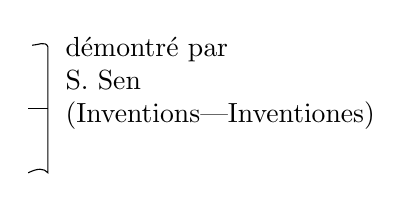
\begin{tikzpicture}[x=1cm,y=1cm]
\draw (0,0) .. controls (.12,.06) and (.2,.06) .. (.25,0) -- (.25,1.6) .. controls (.22,1.68) and (.12,1.62) .. (.05,1.62);
\draw (0,.82)--(.25,.82);
\node[anchor=north west,align=left] at (.35,1.85) {démontré par\\S. Sen\\(\unsure{Inventions|Inventiones})};
\end{tikzpicture}}}

\begin{center}\textbf{Bibliographie}\end{center}

[1] \textsc{Chevalley}, C.: Théorie des groupes de LIE, II et III. Publ. Inst. Math. Univ. Nancago, Paris: Hermann 1951 et 1955.

[2] \textsc{Lubin}, J.: One-parameter formal LIE groups over $p$-adic integer rings. Ann. of Maths. \textbf{80}, 464--484 (1964).

[3] \textsc{Lubin}, J.: Finite subgroups and isogenies of one-parameter formal LIE groups. Ann. of Maths. \textbf{85}, 296--302 (1961).

[4] \textsc{Mumford}, D.: Geometric invariant theory. Ergeb. der Math., Neue Folge, Bd. 34. Berlin, Heidelberg, New York, Springer 1965.

[5] \textsc{Mumford}, D.: Families of abelian varieties. Algebraic groups and discontinuous subgroups. Proc. Symp. Pure Maths. \textbf{9}, A.M.S. (1966).

[6] \textsc{Serre}, J-P.: Corps Locaux. Publ. Inst. Math. Univ. Nancago, VIII, Paris: Hermann 1962.

[7] \textsc{Serre}, J-P.: LIE algebras and LIE groups. New York: Benjamin 1965.

[8] \textsc{Serre}, J-P.: Résumé des cours 1965--66. Annuaire du Collège de France, 49--58, (1966--67).

[9] \textsc{Tate}, J.: $p$-divisible groups, ce volume p. 158--183.
\margin{16}

\scanpage{18}
\begin{center}
EXTRAIT

DE

L'ANNUAIRE DU COLLÈGE DE FRANCE

\rule{1.1cm}{.4pt}

68\textsuperscript{e} ANNÉE

(1968-1969)

\rule{1.1cm}{.4pt}

RÉSUMÉ DES COURS DE 1967-1968

\rule{1.6cm}{.4pt}
\end{center}
\margin{17}

\scanpage{19}
\begin{center}--- 47 ---\end{center}

\begin{center}\textbf{Algèbre et géométrie}

M. Jean-Pierre \textsc{Serre}, professeur\end{center}

Soit $\mathrm K$ un corps complet pour une valuation discrète, de corps résiduel $k$. On suppose que $\mathrm K$ est de caractéristique zéro et que $k$ est algébriquement clos de caractéristique $p$. Soit $\overline{\mathrm K}$ une clôture algébrique de $\mathrm K$, et soit $\mathrm G$ le groupe de Galois de $\overline{\mathrm K}$ sur $\mathrm K$. Soit $\mathrm V$ un espace vectoriel de dimension finie sur le corps $p$-adique $\mathbf Q_p$, et soit
\[
\varrho:\mathrm G\to\operatorname{Aut}(\mathrm V)
\]
un homomorphisme continu. On dit alors que $\mathrm V$ (ou $\varrho$) est une \textit{représentation $p$-adique} de $\mathrm G$.

Soit $\chi$ l'homomorphisme de $\mathrm G$ dans le groupe des unités $p$-adiques correspondant à l'action naturelle de $\mathrm G$ sur les racines de l'unité d'ordre une puissance de $p$. Soit $\mathrm C$ le complété de $\overline{\mathrm K}$. Si $\mathrm V$ est, comme ci-dessus, une représentation $p$-adique de $\mathrm G$, posons $\mathrm V_{\mathrm C}=\mathrm C\otimes\mathrm V$ (le produit tensoriel étant pris sur $\mathbf Q_p$); pour tout $n\in\mathbf Z$, soit $\mathrm V_{\mathrm C}^n$ le $\mathrm K$-sous-espace de $\mathrm V_{\mathrm C}$ formé des éléments $x$ tels que $\varrho(s)x=\chi(s)^nx$ pour tout $s\in\mathrm G$, et soit $\mathrm V_{\mathrm C}(n)=\mathrm C\otimes_{\mathrm K}\mathrm V_{\mathrm C}^n$. D'après un résultat de \textsc{Tate}, la somme directe des $\mathrm V_{\mathrm C}(n)$ s'identifie à un sous-espace vectoriel de $\mathrm V_{\mathrm C}$. On dit que $\mathrm V$ admet une \textit{décomposition de Hodge $p$-adique} (ou que $\mathrm V$ est un \textit{module de Hodge}) si ce sous-espace vectoriel est égal à $\mathrm V_{\mathrm C}$, autrement dit si l'on a:
\[
\mathrm V_{\mathrm C}=\sum_{n\in\mathbf Z}\mathrm V_{\mathrm C}(n).
\]

Soit $\mathrm V$ un tel module, soit $\mathrm G_{\mathrm V}=\varrho(\mathrm G)$ le sous-groupe correspondant de $\operatorname{Aut}(\mathrm V)$, et soit $\mathrm H_{\mathrm V}$ \textit{l'enveloppe algébrique} de $\mathrm G_{\mathrm V}$, autrement dit le plus petit sous-groupe algébrique (sur $\mathbf Q_p$) du groupe linéaire $\mathbf{GL}_{\mathrm V}$ dont le groupe des points contienne $\mathrm G_{\mathrm V}$.

Le sujet du cours a été l'étude du groupe $\mathrm H_{\mathrm V}$, et en particulier la démonstration des résultats suivants:
\margin{18}

\scanpage{20}
\begin{center}--- 48 ---\end{center}
\margin{\figure{\begin{tikzpicture}\draw (0,0)--(.01,.45);\end{tikzpicture}}}

1) Le groupe $\mathrm G_{\mathrm V}$ est un sous-groupe \textit{ouvert} du groupe $\mathrm H_{\mathrm V}(\mathbf Q_p)$ des points de $\mathrm H_{\mathrm V}$ à coefficients dans $\mathbf Q_p$.

Il revient au même de dire que l'algèbre de Lie du groupe analytique $p$-adique $\mathrm G_{\mathrm V}$ est \textit{algébrique}, au sens de Chevalley.

2) La décomposition $\mathrm V_{\mathrm C}=\sum\mathrm V_{\mathrm C}(n)$ définit un homomorphisme
\[
h:\mathbf G_m/_{\mathrm C}\to\mathbf{GL}_{\mathrm V}/_{\mathrm C}
\]
de groupes algébriques sur $\mathrm C$. Soit $\mathrm H_{\mathrm V}^{\unsure{0|\circ}}$ la composante neutre de $\mathrm H_{\mathrm V}$, et soit $\mathrm H_{\mathrm V}^{\unsure{0|\circ}}/_{\mathrm C}$ le sous-groupe de $\mathbf{GL}_{\mathrm V}/_{\mathrm C}$ déduit de $\mathrm H_{\mathrm V}^{\unsure{0|\circ}}$ par extension des scalaires de $\mathbf Q_p$ à $\mathrm C$. Alors \textit{$\mathrm H_{\mathrm V}^{\unsure{0|\circ}}/_{\mathrm C}$ contient le groupe $h(\mathbf G_m/_{\mathrm C})$}, image de $h$.

Lorsque de plus $\mathrm G_{\mathrm V}$ est \textit{résoluble}, on peut caractériser $\mathrm H_{\mathrm V}^{\unsure{0|\circ}}$ comme \textit{le plus petit sous-groupe algébrique} $\mathrm R$ sur $\mathbf Q_p$ de $\mathbf{GL}_{\mathrm V}$ \textit{tel que $\mathrm R/_{\mathrm C}$ contienne $h(\mathbf G_m/_{\mathrm C})$}; c'est l'analogue $p$-adique du \textit{groupe de Mumford-Tate}.

Il est probable que cette caractérisation de $\mathrm H_{\mathrm V}^{\unsure{0|\circ}}$ vaut sans supposer $\mathrm G_{\mathrm V}$ résoluble; on pourrait le prouver si l'on savait que $\mathrm V_{\mathrm C}=\mathrm V_{\mathrm C}(0)$ entraîne que $\mathrm G_{\mathrm V}$ est fini.
\margin{\figure{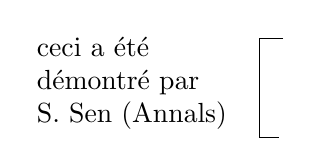
\begin{tikzpicture}[x=1cm,y=1cm]
\node[anchor=north west,align=left] at (0,1.4) {ceci a été\\démontré par\\S. Sen (Annals)};
\draw (3.25,1.25)--(2.95,1.25)--(2.95,0)--(3.2,0);
\end{tikzpicture}}}

3) Lorsque $\mathrm V$ varie, les groupes $\mathrm H_{\mathrm V}$ forment un système projectif; leur limite projective est un \textit{groupe proalgébrique} $\mathrm H$ sur $\mathbf Q_p$, muni d'un homomorphisme $h:\mathbf G_m/_{\mathrm C}\to\mathrm H/_{\mathrm C}$. La catégorie des modules de Hodge est équivalente à celle des $\mathrm H$-modules de dimension finie; si $\mathrm H^{\unsure{0|\circ}}$ désigne la composante neutre de $\mathrm H$, le groupe $\mathrm H/\mathrm H^{\unsure{0|\circ}}$ est le groupe de dimension zéro associé au groupe profini $\mathrm G$; le groupe $\mathrm H^{\unsure{0|\circ}}$ ne change pas lorsqu'on remplace $\mathrm K$ par une extension finie.

4) Soit $\Theta$ le plus grand quotient commutatif du groupe proalgébrique $\mathrm H^{\unsure{0|\circ}}$. Le groupe $\Theta$ est une limite projective de tores; il ne dépend que de $p$ (mais pas de $\mathrm K$); on a:
\[
\Theta=\underset{\leftarrow}{\lim.}\,\mathrm T_{\mathrm E}
\]
où $\mathrm E$ parcourt l'ensemble des extensions finies de $\mathbf Q_p$.

(Si $\mathrm E$ est une extension de $\mathbf Q_p$ de degré $n$, on note $\mathrm T_{\mathrm E}$ le tore $\mathrm R_{\mathrm E}/_{\mathbf Q_p}(\mathbf G_m/_{\mathrm E})$ défini par $\mathrm E$; sa dimension est $n$, et $\mathrm T_{\mathrm E}(\mathbf Q_p)$ est canoniquement isomorphe à $\mathrm E^*$.)

Ce résultat est essentiellement équivalent à un théorème exposé par \textsc{Tate} dans le séminaire 1965/66. Il est intimement lié aux propriétés des «multiplications complexes formelles» des groupes $p$-divisibles.
\margin{19}

\scanpage{21}
\begin{center}--- 49 ---\end{center}
\margin{\figure{\begin{tikzpicture}\draw (0,0)--(0,.45);\end{tikzpicture}}}

5) Faisons maintenant l'hypothèse que $\mathrm V$ ne fait intervenir que les exposants 0 et 1, autrement dit que $\mathrm V_{\mathrm C}=\mathrm V(0)+\mathrm V_{\mathrm C}(1)$; posons
\[
n_0=\dim_{\mathrm C}\mathrm V_{\mathrm C}(0)\text{ et }n_1=\dim_{\mathrm C}\mathrm V_{\mathrm C}(1).
\]
(Le module $p$-adique attaché à un groupe $p$-divisible est de ce type, l'entier $n_1$ étant égal à la dimension du groupe.)

Supposons que $n_1=1$ et que $\mathrm V$ soit un $\mathrm H_{\mathrm V}^{\unsure{0|\circ}}$-module simple. Alors le commutant de $\mathrm H_{\mathrm V}^{\unsure{0|\circ}}$ dans $\operatorname{End}(\mathrm V)$ est un corps commutatif $\mathrm E$ de degré fini sur $\mathbf Q_p$, et $\mathrm H_{\mathrm V}^{\unsure{0|\circ}}$ est égal au groupe algébrique des $\mathrm E$-automorphismes de $\mathrm V$; il en résulte, conformément à ce qu'avaient conjecturé \textsc{Lubin} et \textsc{Tate}, que le groupe $\mathrm G_{\mathrm V}$ contient un sous-groupe \textit{ouvert} de $\operatorname{Aut}_{\mathrm E}(\mathrm V)$.

Le cours s'est achevé par un essai de classification dans le cas $n_1>1$ (en supposant $\mathrm V$ absolument simple sur $\mathrm H_{\mathrm V}^{\unsure{0|\circ}}$), basé sur le fait que $\mathrm H_{\mathrm V}^{\unsure{0|\circ}}/_{\mathrm C}$ contient un tore de dimension 1 \textit{n'ayant que deux poids}.
\margin{\figure{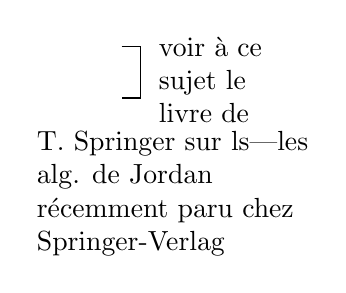
\begin{tikzpicture}[x=1cm,y=1cm]
\draw (0,2.15)--(.24,2.15)--(.24,1.5)--(0,1.5);
\node[anchor=north west,align=left] at (.35,2.4) {voir à ce\\sujet le\\livre de};
\node[anchor=north west,align=left] at (-1.2,1.2) {T. Springer sur \unsure{ls|les}\\alg. de Jordan\\récemment paru chez\\Springer-Verlag};
\end{tikzpicture}}}

\begin{center}\textsc{Séminaire}\end{center}

Le séminaire a continué celui de 1965/66, relatif aux \textit{groupes $p$-divisibles}. Il a comporté neuf exposés: quatre par Michel \textsc{Raynaud} et cinq par John \textsc{Tate} (qui en avait fait dix en 1965/66).

Michel \textsc{Raynaud} a rappelé les notions préliminaires nécessaires: schémas en groupes finis, dualité de Cartier, quotients. Il a ensuite donné la définition des groupes $p$-divisibles, et montré leur interprétation comme groupes formels. Dans son dernier exposé, il a démontré le théorème fondamental, dû à \textsc{Tate}, qui affirme que, en inégale caractéristique, le passage de l'anneau des entiers au corps des fractions définit un foncteur \textit{pleinement fidèle} sur la catégorie des groupes $p$-divisibles. Il est possible que sa démonstration, différente de celle de \textsc{Tate}, puisse être adaptée au cas d'égale caractéristique.

Les exposés de John \textsc{Tate} ont eu pour thème le \textit{théorème de relèvement} des variétés abéliennes, autrement dit le fait que relever une variété abélienne revient à relever le groupe $p$-divisible correspondant (la caractéristique résiduelle étant égale à $p$). A Woods Hole, en 1964, \textsc{Tate} en avait donné une démonstration basée sur une certaine construction cohomologique. Dans le séminaire, il a proposé une autre méthode, où variété abéliennes et groupes $p$-divisibles n'interviennent que par les \textit{faisceaux} correspondants (pour des topologies d'\textsc{Artin-Grothendieck} convenables). Cette méthode, malgré des difficultés techniques qui n'ont pas été entièrement résolues, paraît plus naturelle que la précédente, et de portée plus générale.

4
\margin{20}

\scanpage{22}
\begin{center}--- 50 ---\end{center}

Un cas particulier intéressant est celui où la variété abélienne est \textit{ordinaire}, autrement dit a le maximum possible de points d'ordre $p$. Il existe alors un \textit{relèvement canonique} que l'on peut caractériser de diverses manières; dans le cas des courbes elliptiques, ce relèvement avait été signalé en 1933 par H. \textsc{Hasse} (qui se plaçait à un point de vue quelque peu différent).

\begin{center}\textsc{Publications}\end{center}

H. \textsc{Bass}, J. \textsc{Milnor} et J.-P. \textsc{Serre}, \textit{Solution of the congruence subgroup problem for $\mathrm{SL}_n$ $(n\geq3)$ and $\mathrm{Sp}_{2n}$ $(n\geq2)$} (\textit{Publ. Math. I.H.E.S.}, n\textsuperscript{o} 33, 1967, p. 59-137).

J.-P. \textsc{Serre}, \textit{Local Class Field Theory}; \textit{Complex Multiplication} (chap. VI et XIII de J. \textsc{Cassels} et A. \textsc{Fröhlich}, \textit{Algebraic Number Theory}, Acad. Press, New York, 1967).

--- \textit{Sur les groupes de Galois attachés aux groupes $p$-divisibles} (\textit{Proc. Conf. Local Fields}, Driebergen, 1966, Springer-Verlag, p. 118-131).

--- \textit{Commutativité des groupes formels de dimension 1} (\textit{Bull. Sci. math.}, 91, 1967, p. 113-115).

--- \textit{Représentations linéaires des groupes finis} (Paris, Hermann, 1968).

--- \textit{Abelian $l$-adic representations and elliptic curves} (Notes rédigées avec la collaboration de W. \textsc{Kuyk} et J. \textsc{Labute}, W. A. Benjamin Publ., New York, 1968).

\begin{center}\textsc{Missions}\end{center}

Cours à McGill University, Montréal (septembre 1967).

Conférences à l'Université de Montréal (septembre 1967), à Haverford College (octobre 1967), à l'Institute for Advanced Study de Princeton (octobre-décembre 1967) et à l'Université de Grenoble (juin 1968).
\margin{21}

\scanpage{23}
\deleted{$\unsure{K|k}$} $K$ corps local d'inégales caractéristiques, corps résiduel $k$ de car. $p>0$ ($k$ parfait!), anneau d'entiers $V$, sous-$p$-anneau $W$ de corps résiduel $k$, corps des fractions $L$. On choisit une clôture algébrique $\overline K\deleted{\unsure{\Omega}}$ de $K$, son complété $\Omega$.
\margin{\diagram{\begin{array}{ccccccc}
L&\subset&K&\subset&\overline K&\subset&\Omega\\
\cup&&\cup&&\cup&&\cup\\
W&\subset&V&\subset&\overline V&\subset&\widehat{\overline V}
\end{array}}}

On pose
\[
\pi=\operatorname{Gal}(\overline K/K),\quad\pi'=\operatorname{Gal}(\overline K/L)\ldots
\]

$\mathcal M_K=$ catégorie des \inserted{$Q_p$-}faisceaux de type Hodge-Tate sur $K$
\inserted{($\otimes$-catégorie sur $Q_p$)}
\[
\mathcal M_K^+=\unsure{\underline{\lim}|\varinjlim}\mathcal M^{(\unsure{n|u})};
\]
ss-catégorie des objets ``effectifs'' i.e. avec \deleted{\unsure{à graduation}} $\operatorname{gr}(M_\Omega)$ à degrés positifs
\[
\mathcal M_K^{(\unsure{u|1})}=\{\text{\unsure{ss-catégorie} pleine \unsure{de|en} $\mathcal M$ formée des $M$ avec $\operatorname{gr}M_\Omega$ à degrés 0 et 1}
\]

$\widetilde{\mathrm{BT}}_{\unsure{V}}$ catégorie des BT à isog. près \uline{sur $V$}

Foncteur pl. fid (par Tate)
\diagram{\begin{tikzcd}
\widetilde{\mathrm{BT}}_V\arrow[r,hook]&\mathcal M_K^{(\unsure{u|1})}
\end{tikzcd}}
\margin{on identifie $\widetilde{\mathrm{BT}}_V$ à ss-catégorie \unsure{pleine} de $\mathcal M_K^{(\unsure{u|1})}$}

$\mathcal M_{\unsure{K}\deleted{\unsure{+|\Omega}}}^{\mathrm{BT}}\unsure{\in|\subset}\mathcal M_K$ $\otimes$-\deleted{\unsure{ss}}catégorie Tannakienne engendrée par $\mathcal M_K^{(1)}$

\diagram{\begin{tikzcd}
T_p^\Omega=T_p:\mathcal M_K\arrow[r]&\deleted{\unsure{\operatorname{Rep}(\pi,Q_p)|\operatorname{Modf}(Q_p)}}\operatorname{Modf}(Q_p)
\end{tikzcd}}
foncteur fibre en $\Omega$
\[
G^\Omega=G^{\deleted{\unsure{\Omega}}}=\operatorname{Aut}(T_p)\qquad\text{pro-groupe \unsure{alg.} sur }Q_p
\]

\diagram{\begin{tikzcd}\pi\arrow[r,"\rho"]&G(Q_p)\end{tikzcd}}
$G$ est l'enveloppe algébrique de $\pi$

(NB $G/G^0$ \unsure{non} tordu)\unsure{!}

Pour $M\in\operatorname{Ob}\mathcal M$, $G_M=\operatorname{Im}(G\to\underline{\operatorname{Aut}}_{Q_p}(T_p(M)))\subset\underline{\operatorname{Aut}}_{Q_p}(T_p(M))$
\diagram{\begin{tikzcd}
(\pi_{\deleted{\unsure{K|M}}}\arrow[r,"\rho_M"]&G_M(Q_p)\quad\ldots\ldots)
\end{tikzcd}}

\diagram{\begin{array}{cccc}
\begin{gathered}\text{Structure}\\\text{sur }(\Omega,\pi)\end{gathered}&
\begin{tikzcd}[column sep=small,row sep=small]&G_\Omega^!\\G_{m\Omega}\arrow[ur,"j^!"]&\end{tikzcd}&
\begin{gathered}\Phi\\\text{avec section }e\\\text{sur }\Omega\\\text{\unsure{pas invariante|par invariants}}\\\text{sous }\pi\end{gathered}&G_\Omega\\[1em]
\text{id}&
\begin{tikzcd}[column sep=small,row sep=small]&G_\Omega^{\mathrm{Hdg}}\\G_{m\Omega}\arrow[ur,"j_\Omega"]&\end{tikzcd}&
Q_\Omega=\tau\mathop{\wedge}_{G_{m\Omega}}\Phi&G_\Omega\\[1em]
\begin{gathered}\text{par descente}\\\text{sur }K\end{gathered}&
\begin{tikzcd}[column sep=small,row sep=small]&G_K^{\mathrm{Hdg}}\\G_{mK}\arrow[ur,"j_K"]&\end{tikzcd}&Q_K&G_K
\end{array}}
\margin{$[\tau\inserted{=\tau^\Omega}$ $G_{m\Omega}$-tors, sur $(\Omega,\pi)$ associé à $T_p(\Omega^*)\otimes_{\mathbf Z_p}\Omega]$}
\[
T_{\mathrm{Hdg}}^{\deleted{\unsure{K|\Omega}}}(M)=Q_K\mathop{\wedge}_G M_K
\]

Pour $M\in\operatorname{Ob}\widetilde{\mathrm{BT}}_V$, on a \deleted{\unsure{sur} $T_{\mathrm{Hdg}}(M)$} un

\unsure{a)|1\textsuperscript{o})} Un $\unsure{L|K}$-vectoriel \deleted{\unsure{filtré}} $T_{\unsure{\mathrm{DR}|\mathrm{DE}}}(M)$ \deleted{et un isom
\[
\operatorname{gr}T_{\mathrm{DR}}(M)_K\unsure{\sim|\simeq}T_{\mathrm{Hdg}}(M)
\]}
\margin{22}

\scanpage{24}
b) Une \deleted{\unsure{donnée}} \inserted{structure} de $F$-\inserted{iso}cristal sur $T_{\mathrm{cr}}(M)$

c) Une filtration \unsure{de|sur} $T_{\mathrm{DR}}(M)=T_{\mathrm{cr}}(M)\otimes_K L$

d) Un isomorphisme
\[
\operatorname{gr}(T_{\mathrm{DR}}(M))\simeq T_{\mathrm{Hdg}}(M)
\]

ces données étant fonctorielles en $M\in\operatorname{Ob}\widetilde{\mathrm{BT}}_{\unsure{V}}$

\uline{Question} Peut-on prolonger ces données à $\mathcal M^{\mathrm{BT}}$, \deleted{\unsure{?} \unsure{A-t-on}}

avec $T_{\mathrm{cr}}$ un $\otimes$-foncteur, \unsure{la|le} structure b) \unsure{compatible|compatibles} avec $\otimes$ \inserted{et Hom}, c) et d) aussi. A-t-on unicité de $T_{\mathrm{cr}}$ prolongé, à isom unique près?
\margin{\figure{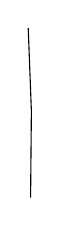
\begin{tikzpicture}\draw (0,2.15)--(.04,1.1)--(.03,0);\end{tikzpicture}}}
\margin{23}

\scanpage{25}
1) gr. alg $\boxed{G}$ sur $\mathbf Q_p$.

2) hom continu
\[
\boxed{\rho:\pi\mathrel{\unsure{-|\longrightarrow}}G(\mathbf Q_p)}
\]
d'où
\diagram{\begin{tikzcd}[column sep=small,row sep=small]
& \unsure{Q|\Phi}_\Omega^! \arrow[dl,dash] \arrow[dr,dash] & \\
G_\Omega^! &&G_\Omega
\end{tikzcd}}

\margin{unique}
\margin{\deleted{\unsure{fg}}}
\figure{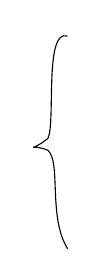
\begin{tikzpicture}[x=1cm,y=1cm]
\draw (0.3,2.7) .. controls (0,2.8) and (0.15,1.6) .. (0.05,1.4)
 .. controls (-0.2,1.2) and (-0.2,1.35) .. (0.05,1.25)
 .. controls (0.22,1.1) and (0.05,0.4) .. (0.3,0);
\end{tikzpicture}}
3)
\[
\boxed{G_{m\Omega}\xrightarrow{j^!}G_\Omega^!}
\]
d'où
\diagram{\begin{tikzcd}[column sep=small,row sep=large]
& Q_\Omega=\tau\wedge_{G_{m\Omega}}\unsure{Q|\Phi}_\Omega^! \arrow[dl,dash] \arrow[dr,dash] & \\
G''_\Omega=(\tau^{\unsure{*}}\wedge_{G_{m\Omega}}(G_\Omega^!,\mathrm{int})) && G_\Omega
\end{tikzcd}}
\[
\overbrace{j_\Omega:G_m\longrightarrow G''_\Omega}
\]

4) $\boxed{Q_L\text{ sur }G_L}$ descendant $Q_\Omega$ sur $G_\Omega$.
\diagram{\begin{tikzcd}[column sep=small]
U''_L\subset G''_L \arrow[r,dash] & Q_L \arrow[r,dash] & G_L
\end{tikzcd}}
\[
,\quad j_L:G_{mL}\mathrel{\unsure{-|\longrightarrow}}G''_L
\]

5) \deleted{Un \unsure{ensemble} $\boxed{\Delta}$ d'opérations
\inserted{\figure{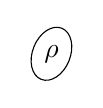
\begin{tikzpicture}[baseline=-.4ex]\draw[rotate=-22] (0,0) ellipse (.24 and .35);\node at (0,0) {$\rho$};\end{tikzpicture}}} de $\Gamma\ (\supset\pi)$ sur $Q_\Omega$
\margin{\unsure{commutant}}
\inserted{d'où $\Gamma\longrightarrow G''_L(\Omega)=G''_\Omega(\Omega)$}
\unsure{prolongeant} celle de $\pi$, \unsure{comp.} avec celle de $\Gamma$ sur $\Omega$

tel que si $\rho$ \unsure{est telle}, \unsure{par des} \unsure{formant} orbite sous $U''_L$
opérant par (pour $u\in U''_L(L)$)
\[
(u.\rho)(\gamma)=\tau u\{\rho(\gamma)\}\tau u^{-1}
=\unsure{(\mathrm{int}\,\tau(u)).\rho(\gamma)|(\mathrm{int}\,\tau(u).\rho)(\gamma)}
\]
i.e.
\[
\unsure{u-\rho|u.\rho}=\mathrm{int}\,\tau(u)\rho)
\]
[NB si $u\rho=\rho$ i.e. $\deleted{\unsure{\tau u.\rho}}\ \rho$ commutant à $\tau(u)$ pour
\margin{\unsure{donc|pour}}
}
\figure{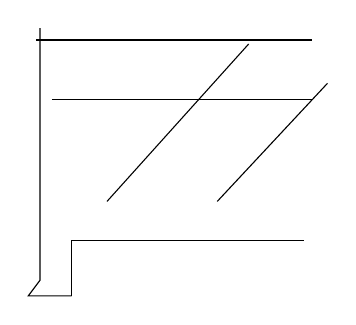
\begin{tikzpicture}[x=1cm,y=1cm]
\draw (0.15,3.4)--(0.15,0.2)--(0,0)--(0.55,0);
\draw (0.55,0)--(0.55,0.7)--(3.5,0.7);
\draw (0.1,3.25)--(3.6,3.25);
\draw (0.3,2.5)--(3.6,2.5);
\draw (1,1.2)--(2.8,3.2);
\draw (2.4,1.2)--(3.8,2.7);
\end{tikzpicture}}

Un torseur (\unsure{non nullité}) \inserted{à droite $\uline{\Delta}$}
$\unsure{R_0|P_0}$ sous $U''_L(L)$, et
un $U''_L(L)$-\uline{hom de}
\diagram{\begin{tikzcd}[column sep=large]
\rho:\Delta\arrow[r] &
\begin{array}{l}
\mathrm{Op.}\text{ de }\Gamma\text{ sur }(\Omega,Q_L,G_L)\\
\text{qui sont compatibles avec}\\
\text{\unsure{l'op. donnée|l'op. qui}}\text{ de }\Gamma\text{ sur }\Omega,\\
\text{et celle de }\pi\unsure{\in|\subset}\Gamma\text{ sur }Q_L\ldots
\end{array}
\end{tikzcd}}
\figure{\begin{tikzpicture}[x=1cm,y=1cm]
\draw (0.1,1.6)..controls (0,1.5) and (0,0.2)..(0,0)--(2.3,0);
\end{tikzpicture}}
lorsque on fait opérer $U''_L(L)$ \inserted{à droite} sur le deuxième ens. par
\[
u.\alpha=\tau(\alpha)u\tau(\alpha)^{-1}
\]
\margin{24}

\scanpage{26}
1) groupe alg. $\boxed{G}$ sur $\mathbf Q_p$.
(Il dépend en fait du choix de $\Omega$. cf plus bas 2°)

2) Hom
\[
\boxed{\rho:\pi\longrightarrow G(\mathbf Q_p)}
\]
[L'op. de $\pi=\operatorname{Aut}_L(\Omega)$ sur $G=G^{(\Omega)}$ est donnée par
$\sigma\longmapsto\mathrm{int}(\rho(\sigma))$

\deleted{3)} On fait opérer $\pi$ sur $G_\Omega$ \uline{diagonalement}, soit $G_\Omega^!$.

3) Hom
\[
\boxed{j^!_{\unsure{\Omega}}:G_{m\Omega}\longrightarrow G_\Omega^!}
\]
\margin{inv. par $\pi$}
\margin{$G_\Omega^{\unsure{!|1}}$}

On appelle \deleted{$\unsure{S_\Omega(1)|S(1)}$}\inserted{$S_\Omega$}
\deleted{$\unsure{T_\Omega}$} le \deleted{$\unsure{T}$}
$\Omega$-module inversible $T_p(\Omega)^{\unsure{*|\#}}\otimes_{\mathbf Z_p}\Omega$
avec op. diagonale de $\pi$, \deleted{\illegible{1}} et $\tau_\Omega$ le $G_{m\Omega}$ torseur associé.
Posons
\deleted{\[
\tau\wedge_{\unsure{G_{m\Omega}}}\Phi
\unsure{\wedge}_{G_{m\Omega}}\unsure{G_\Omega^!}\quad
\unsure{Q_\Omega}\ \unsure{=\tau}\wedge_{\unsure{G_{m\Omega}}}\unsure{G_\Omega^!}
\]}
\inserted{\figure{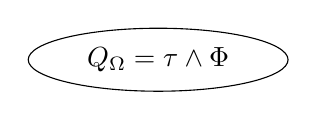
\begin{tikzpicture}
\node at (1.6,0) {$Q_\Omega=\tau\wedge\Phi$};
\draw (1.6,0) ellipse (1.65 and 0.4);
\end{tikzpicture}}}
torseur \inserted{à dr} sur $G_\Omega$
\[
\text{d'où}\quad \uline{G_\Omega^!\text{ tordu}}\text{ par }(\tau,j),
\quad\text{soit }\figure{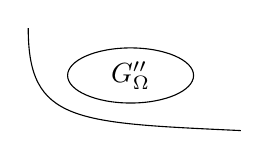
\begin{tikzpicture}[baseline=0pt]
\node at (0.8,0.3) {$G''_\Omega$};
\draw (0.8,0.3) ellipse (0.8 and 0.35);
\draw (-0.5,0.9) .. controls (-0.5,-0.3) and (0.1,-0.3) .. (2.2,-0.4);
\end{tikzpicture}}
\]
[Correspond au foncteur fibré \inserted{(gradué)} sur $\operatorname{Rep}(G)$
\diagram{\begin{tikzcd}
G_{m\Omega}\arrow[r,"j_\Omega^{\unsure{*|\#}}"]&G''_\Omega
\end{tikzcd}}
\[
M\longrightarrow\sum\operatorname{gr}_j^i(M)_\Omega\otimes S_\Omega(i)
=\operatorname{Hdg}_\Omega(M)
\]

\margin{$\unsure{\angle|4}$}
\uline{Axiome} Le \deleted{foncteur}\inserted{$(T_{\mathrm{Hdg}})$}
$Q_\Omega$ \deleted{\unsure{sur}} se descend à $L$
en un $G_L$-torseur $Q_L$
\figure{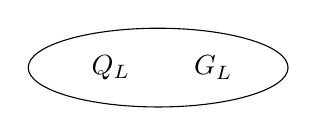
\begin{tikzpicture}
\node at (0.7,0) {$Q_L$};\node at (2,0) {$G_L$};
\draw (1.3,0) ellipse (1.65 and 0.5);
\end{tikzpicture}}
(unique à isom unique près)
en un $G''_L$, et
\diagram{\begin{tikzcd}
G_{mL}\arrow[r,"j_L"]&G''_L
\end{tikzcd}}
Correspond : fct fibré gradué $\operatorname{Hdg}_L$

\margin{\uline{NB} Un $j$ satisfaisant aux conditions est \unsure{unique}.
Signifie que les $\unsure{M_\Omega^!|M_\Omega}$ sont \uline{de Hodge}.
Du moins si}

\figure{\begin{tikzpicture}[x=1cm,y=1cm]
\draw (0,0) .. controls (2,0.4) and (4,-0.2) .. (8,0.1);
\end{tikzpicture}}
\margin{$\unsure{Q|\alpha}$}
Il y a deux foncteurs fibres de $\operatorname{Rep}(G)$ dans $\operatorname{Mod}(\Omega,\pi)$
\[
\begin{array}{ll}
a)\quad M\longrightarrow M_\Omega &
\text{\unsure{opérations|opération} provenant des op. \unsure{canoniques} de }\pi\text{ sur }\Omega\\
b)\quad M\mathrel{-}M_\Omega^! &\text{opération diagonale}
\end{array}
\]
-- foncteurs $T_{p\Omega}$ et $T^!_{p\Omega}$

\deleted{Après oubli des op.} On a là un \deleted{$(\Omega,\pi)$} torseur \inserted{à droite} sur
$(\Omega,\pi)$ de groupe $G_\Omega$, soit $\Phi_\Omega$, donné par le 1-cocycle
\[
\rho:\pi\mathrel{-}G(\mathbf Q_p)\subset H^0(\Omega,\unsure{\deleted{\pi}|\pi};G_\Omega)=G(\unsure{L|\Omega}).
\]
Le \deleted{groupe} $\uline{\operatorname{Aut}}_{G_{\Omega,\pi}}(\Phi)$ est $G_\Omega^!$.
\margin{$(\Omega,\pi)$}
\figure{\begin{tikzpicture}
\draw (0,0) .. controls (0.6,0.1) and (1.5,-0.1) .. (1.7,0.45);
\end{tikzpicture}}
\margin{25}

\scanpage{27}
4) Soit
\figure{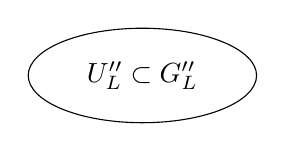
\begin{tikzpicture}
\node at (1.4,0) {$U''_L\subset G''_L$};
\draw (1.4,0) ellipse (1.45 and 0.6);
\end{tikzpicture}}
\uline{défini} par $j_L$. On a un torseur
\inserted{à droite} can (\unsure{uni|mais} trivial)
$\boxed{R_L\text{ sous }U''_L}$, d'où foncteur fibré filtré
\[
\operatorname{DR}_L(M)=\deleted{T_p(M)_L}
(R_L\wedge_{U''_L}Q_L)\wedge_{G_L}T_p(M)_L
\]

\deleted{\unsure{5)}} Le foncteur fibré $\operatorname{DR}_L(M)$ correspond au $G_L$-tors.
\inserted{à dr.}
\figure{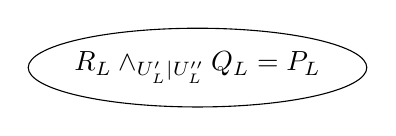
\begin{tikzpicture}
\node at (2,0) {$R_L\wedge_{\unsure{U'_L|U''_L}}Q_L=P_L$};
\draw (2,0) ellipse (2.15 and 0.5);
\end{tikzpicture}}
Soit $\unsure{G''_L|G'_L}=\uline{\operatorname{Aut}}(P_L)$
\[
(G''_L\simeq G'_L\text{ non canonique})
\]

\figure{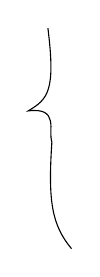
\begin{tikzpicture}[x=1cm,y=1cm]
\draw (0.25,2.8) .. controls (0.35,2) and (0.25,1.9) .. (0,1.75)
 .. controls (0.4,1.8) and (0.25,1.5) .. (0.3,1.35)
 .. controls (0.25,0.6) and (0.3,0.3) .. (0.55,0);
\end{tikzpicture}}
5) \uline{Structure de descente} de $L$ à $K$ \uline{sur le}
\uline{torseur} $P_L$, d'où
\[
\unsure{G''|G'}\quad P_K\quad G_K
\]
6) $G_K$-Isom donné
\[
P_K\simeq P_{\unsure{k|L}}^{(\unsure{f|\phi})}
\]

On peut formuler ensemble 5) et 6) en regardant
\[
P_\Omega=\unsure{R_L^{\leftarrow}|R_L}\wedge_{U''_\Omega}\deleted{\unsure{P}}Q''_\Omega
=R_L\wedge_{U''_\Omega}
\]
et en déclarant que l'ext. $\Gamma$ de $\mathbf Z$ par
$\widetilde\pi=\operatorname{Gal}(\unsure{\bar k/k|\bar K/K})$
(qui contient $\pi\subset\Gamma$) \uline{opère} sur $P_\Omega$ en \unsure{prolongeant}
l'op. \unsure{qu'on a} déjà sur $\pi$.
\margin{26}

\scanpage{28}
On a donc une \uline{extension}
\diagram{\begin{tikzcd}[column sep=small]
1\arrow[r]&G'_S(\unsure{S|\Omega})\arrow[r,dash]&\mathcal E\arrow[r]&\Gamma\arrow[r]&1\arrow[r,dash]&\unsure{0|\circ}
\end{tikzcd}}
\hfill $(\mathcal E)$

\deleted{Supposons que $\pi\unsure{\in|\subset}\Gamma$ opère sur}
\inserted{$\pi$}

Les \uline{sections} de celle-ci sont les structures de torseur sur $(S,\Gamma;G_S)$ sur $Q_S$ qui
\unsure{prolongent} sa structure de tor. sur $(S,G_S)$.
Si on a une telle section, on en déduit une opération de $\Gamma$ sur $G'_S(\unsure{S|\Omega})$
(qui en fait provient de son opération sur $G'_S$ lui-$=$ !)
et les autres sections correspondent aux 1-cocycles de $\Gamma$ à valeurs dans $G'_S(\unsure{S|\Omega})$.
\deleted{Les}\inserted{L'ens $\Gamma(\mathcal E)$ des} sections
forment \deleted{\illegible{1}} un ens où $G'_S(\unsure{S|\Omega})$ opère
(\unsure{autom.|automs} intérieurs) et deux \deleted{\unsure{de pts. de|élts. de}}
$\Gamma(\mathcal E)$ sont
\inserted{conjugués ssi le 1-cocycle faisant passer de l'un à l'autre
\unsure{est coh. à} $1$}.
\figure{\begin{tikzpicture}[x=1cm,y=1cm]
\draw (0,0) .. controls (-0.15,0.4) and (1.7,0.7) .. (2,0.8);
\draw (0.1,0.5)--(0.3,0.3)--(0.4,0.55);
\end{tikzpicture}}

Si on a un \unsure{ss-gr|sous-gr} $\pi\subset\Gamma$ et une section
$\alpha_0:\pi\longrightarrow\mathcal E$ partielle, on peut s'intéresser
à l'ens des $g\in G'_S(\unsure{S|\Omega})$ qui la fixent, c'est \unsure{l'ens} des
élts de $G'_S(\unsure{S|\Omega})$ fixés par $\pi$ (y opérant comme de juste)
$G'_S(\unsure{S|\Omega})^\pi\ (=G'_L(L))$.
Les sections $\alpha$ qui prolongent $\alpha_0$ sont donc telles que
$G'_S(\unsure{S|\Omega})^\pi$ y opère, Si on a
\margin{27}

\scanpage{29}
un tel $\alpha$, les autres $\beta$ s'en déduisent par les 1-cocycles qui sont
\uline{triviaux} sur $\pi$,
\[
\left\{\begin{array}{l}
\varphi(\sigma\sigma')=\varphi(\sigma){}^\sigma\varphi(\sigma')\\
\varphi(\pi)=\{e\}
\end{array}\right.
\]

\uline{Question} Est-il vrai que les $\alpha$ qui prolongent $\alpha_0$ sont
\unsure{coh.|ch.} i.e. conjugués sous $G'_S(S)$ ?
il suffirait de savoir que pour une telle section (fixée)
\[
H^1(\Gamma,G'_S(S))\mathrel{-}H^1(\pi,G'_S(S))
\]
est injectif (ou \unsure{fblt|fbt} injectif, i.e. noyau nul)
Si oui, les solutions cherchées forment un
\deleted{torseur}\inserted{\unsure{esp. homogène}}
sous $G'_S(S)^\pi\ (=G'_L(L))$

\figure{\begin{tikzpicture}[x=1cm,y=1cm]
\draw (0,3.4)--(0,2.8);
\draw (0,2.45) .. controls (0.15,2.15) and (-0.1,1.9) .. (0.05,1.55);
\draw (0.05,1.1)--(0.05,0);
\draw (0.65,1.5)--(0.53,0.75);
\draw (0.7,1.5)--(0.58,0.75);
\draw (0.75,1.5)--(0.63,0.75);
\end{tikzpicture}}
\figure{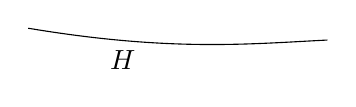
\begin{tikzpicture}[x=1cm,y=1cm]
\draw (0,0.35) .. controls (1.8,0.05) and (2.8,0.15) .. (3.8,0.2);
\node at (1.2,-0.05) {$H$};
\end{tikzpicture}}
\figure{\begin{tikzpicture}[x=1cm,y=1cm]
\draw (2.3,10.5)--(1.4,4.5)--(1.35,0);
\draw (1.55,4.5) .. controls (0.2,3.85) and (0.3,3.65) .. (1.85,4.25)
 .. controls (2.5,4.5) and (0.6,3.35) .. (1.3,3.55)
 .. controls (2.8,4) and (2.5,3.5) .. (1.05,2.5)
 .. controls (0.4,2.05) and (1.65,2.4) .. (1.7,1.8)
 .. controls (1.8,1.2) and (1.3,1) .. (1.5,0.55);
\end{tikzpicture}}

\diagram{\begin{tikzcd}
\mathbf Q_p\arrow[r,dash]&K
\end{tikzcd}}
\[
T_K(\deleted{\unsure{K}})=\prod_{K/\mathbf Q_p}G_m
\]
\margin{$\displaystyle\prod_{\unsure{o|\mathcal O}/\mathbf Z_p}\unsure{G_m}$}
\diagram{\begin{tikzcd}
{}\arrow[r]&T_{\unsure{o_K|\mathcal O_K}}\arrow[r]&\mathbf Z\arrow[r]&0
\end{tikzcd}}

\diagram{\begin{tikzcd}[column sep=small,row sep=large]
&&&&\text{Modèle de Nér. de }g_K&\\
&0\arrow[r]&g_{\unsure{0|o}}\arrow[r]&N\arrow[r]\arrow[ur,dash]&\mathbf Z_{\unsure{0|o}}\arrow[r]&0\\
\unsure{m|\text{sur}}&0\arrow[r]&g_{\unsure{0|o}}\arrow[r]\arrow[u,Rightarrow]&\widetilde N\arrow[r]\arrow[u]&\mathbf Z_{\unsure{o|0}}\arrow[r]\arrow[u]&0\\
\begin{array}{c}\unsure{m|\text{sur}}\otimes_{\unsure{o|0}}K\\\Vert\\K\end{array}
&0\arrow[r]&g_K\arrow[r]&\begin{array}{c}\widetilde N_K\\\wr\\g_K\times\mathbf Z_K\end{array}\arrow[r]&\mathbf Z_K\arrow[r]&0
\end{tikzcd}}

\diagram{\begin{tikzcd}[column sep=large,row sep=large]
0&&0\\
\mathbf Z\arrow[u]&&\mathbf Z\arrow[u]\\
T_K(\mathbf Q_p)\simeq K^*\arrow[u]&\unsure{m|\text{sur}}&{}\arrow[u]\\
\unsure{o_K|\mathcal O_K}^*\arrow[u]&&\\
0\arrow[u]&&
\end{tikzcd}}
\diagram{\begin{tikzcd}[column sep=large,row sep=large]
\Gamma(N)\arrow[r,"\sim"]&\Gamma(g)=K^*\arrow[ddl,"\pi"]\\
\Gamma(\widetilde N)\arrow[u,"\unsure{2|?}"]\arrow[d,leftrightarrow]&\\
\begin{array}{c}\Gamma(\widetilde N_K)\\\wr\\\unsure{K^*|gK^*}\times\mathbf Z\end{array}&
\end{tikzcd}}
\margin{28}
